\documentclass[11pt,preprint, authoryear]{elsarticle}

\usepackage{lmodern}
%%%% My spacing
\usepackage{setspace}
\setstretch{1.2}
\DeclareMathSizes{12}{14}{10}{10}

% Wrap around which gives all figures included the [H] command, or places it "here". This can be tedious to code in Rmarkdown.
\usepackage{float}
\let\origfigure\figure
\let\endorigfigure\endfigure
\renewenvironment{figure}[1][2] {
    \expandafter\origfigure\expandafter[H]
} {
    \endorigfigure
}

\let\origtable\table
\let\endorigtable\endtable
\renewenvironment{table}[1][2] {
    \expandafter\origtable\expandafter[H]
} {
    \endorigtable
}


\usepackage{ifxetex,ifluatex}
\usepackage{fixltx2e} % provides \textsubscript
\ifnum 0\ifxetex 1\fi\ifluatex 1\fi=0 % if pdftex
  \usepackage[T1]{fontenc}
  \usepackage[utf8]{inputenc}
\else % if luatex or xelatex
  \ifxetex
    \usepackage{mathspec}
    \usepackage{xltxtra,xunicode}
  \else
    \usepackage{fontspec}
  \fi
  \defaultfontfeatures{Mapping=tex-text,Scale=MatchLowercase}
  \newcommand{\euro}{€}
\fi

\usepackage{amssymb, amsmath, amsthm, amsfonts}

\def\bibsection{\section*{References}} %%% Make "References" appear before bibliography


\usepackage[round]{natbib}

\usepackage{longtable}
\usepackage[margin=2.3cm,bottom=2cm,top=2.5cm, includefoot]{geometry}
\usepackage{fancyhdr}
\usepackage[bottom, hang, flushmargin]{footmisc}
\usepackage{graphicx}
\numberwithin{equation}{section}
\numberwithin{figure}{section}
\numberwithin{table}{section}
\setlength{\parindent}{0cm}
\setlength{\parskip}{1.3ex plus 0.5ex minus 0.3ex}
\usepackage{textcomp}
\renewcommand{\headrulewidth}{0.2pt}
\renewcommand{\footrulewidth}{0.3pt}

\usepackage{array}
\newcolumntype{x}[1]{>{\centering\arraybackslash\hspace{0pt}}p{#1}}

%%%%  Remove the "preprint submitted to" part. Don't worry about this either, it just looks better without it:
\makeatletter
\def\ps@pprintTitle{%
  \let\@oddhead\@empty
  \let\@evenhead\@empty
  \let\@oddfoot\@empty
  \let\@evenfoot\@oddfoot
}
\makeatother

 \def\tightlist{} % This allows for subbullets!

\usepackage{hyperref}
\hypersetup{breaklinks=true,
            bookmarks=true,
            colorlinks=true,
            citecolor=blue,
            urlcolor=blue,
            linkcolor=blue,
            pdfborder={0 0 0}}


% The following packages allow huxtable to work:
\usepackage{siunitx}
\usepackage{multirow}
\usepackage{hhline}
\usepackage{calc}
\usepackage{tabularx}
\usepackage{booktabs}
\usepackage{caption}


\newenvironment{columns}[1][]{}{}

\newenvironment{column}[1]{\begin{minipage}{#1}\ignorespaces}{%
\end{minipage}
\ifhmode\unskip\fi
\aftergroup\useignorespacesandallpars}

\def\useignorespacesandallpars#1\ignorespaces\fi{%
#1\fi\ignorespacesandallpars}

\makeatletter
\def\ignorespacesandallpars{%
  \@ifnextchar\par
    {\expandafter\ignorespacesandallpars\@gobble}%
    {}%
}
\makeatother

\newlength{\cslhangindent}
\setlength{\cslhangindent}{1.5em}
\newenvironment{CSLReferences}%
  {\setlength{\parindent}{0pt}%
  \everypar{\setlength{\hangindent}{\cslhangindent}}\ignorespaces}%
  {\par}


\urlstyle{same}  % don't use monospace font for urls
\setlength{\parindent}{0pt}
\setlength{\parskip}{6pt plus 2pt minus 1pt}
\setlength{\emergencystretch}{3em}  % prevent overfull lines
\setcounter{secnumdepth}{5}

%%% Use protect on footnotes to avoid problems with footnotes in titles
\let\rmarkdownfootnote\footnote%
\def\footnote{\protect\rmarkdownfootnote}
\IfFileExists{upquote.sty}{\usepackage{upquote}}{}

%%% Include extra packages specified by user
\usepackage{graphicx}
\usepackage{epstopdf}
\usepackage{caption}
\usepackage{subcaption}
\usepackage[flushleft]{threeparttable}
\usepackage{threeparttablex}
\usepackage[export]{adjustbox}

%%% Hard setting column skips for reports - this ensures greater consistency and control over the length settings in the document.
%% page layout
%% paragraphs
\setlength{\baselineskip}{12pt plus 0pt minus 0pt}
\setlength{\parskip}{12pt plus 0pt minus 0pt}
\setlength{\parindent}{0pt plus 0pt minus 0pt}
%% floats
\setlength{\floatsep}{12pt plus 0 pt minus 0pt}
\setlength{\textfloatsep}{20pt plus 0pt minus 0pt}
\setlength{\intextsep}{14pt plus 0pt minus 0pt}
\setlength{\dbltextfloatsep}{20pt plus 0pt minus 0pt}
\setlength{\dblfloatsep}{14pt plus 0pt minus 0pt}
%% maths
\setlength{\abovedisplayskip}{12pt plus 0pt minus 0pt}
\setlength{\belowdisplayskip}{12pt plus 0pt minus 0pt}
%% lists
\setlength{\topsep}{10pt plus 0pt minus 0pt}
\setlength{\partopsep}{3pt plus 0pt minus 0pt}
\setlength{\itemsep}{5pt plus 0pt minus 0pt}
\setlength{\labelsep}{8mm plus 0mm minus 0mm}
\setlength{\parsep}{\the\parskip}
\setlength{\listparindent}{\the\parindent}
%% verbatim
\setlength{\fboxsep}{5pt plus 0pt minus 0pt}



\begin{document}



\begin{frontmatter}  %

\title{Replication of `A Reconsideration of Money Growth Rules' by
Belongia \& Ireland (\protect\hyperlink{ref-belongia2020}{2020})}

% Set to FALSE if wanting to remove title (for submission)




\author[Add1]{Tian Cater}
\ead{19025831@sun.ac.za}





\address[Add1]{Advanced time series 2022 Part III project: Baysian
analysis of DSGE models\footnote{\emph{Submitted to Professor Guangling
  Liu, University of Stellenbosch.}}}
\address[Add2]{January 2023}


\begin{abstract}
\small{
This project replicates the New Keynesian model composed by Belongia \&
Ireland (\protect\hyperlink{ref-belongia2020}{2020}), estimated using
Bayesian techniques, to reflect the recent post-financial-crisis episode
of zero nominal interest rates in the US, and demonstrates the effects
of substituting the Federal Reserve's traditional policy of managing
interest rates with the alternative of money growth targeting. In
addition, the sample is extended to the most recent data available to
test the robustness of the findings. For both the benchmark and extended
sample, counterfactual simulations illustrate similar findings to
Belongia \& Ireland (\protect\hyperlink{ref-belongia2020}{2020}); a rule
for modifying the money growth rate modestly and gradually in response
to deviations in the output gap has performance levels comparable to the
calibrated interest rate rule in stabilising inflation and output.
Additionally, the impulse responses disclose that, under the same money
growth rule, the US's post-2008 crisis economic recovery would have been
accelerated due to a significantly shorter period of near-zero nominal
interest rates. These findings insinuate that, with a binding zero lower
bound constraint, policy rules for money growth can provide a simplistic
method for monetary policy to reduce the uneasiness of monetary policy
efficacy.
}
\end{abstract}

\vspace{1cm}





\vspace{0.5cm}

\end{frontmatter}



%________________________
% Header and Footers
%%%%%%%%%%%%%%%%%%%%%%%%%%%%%%%%%
\pagestyle{fancy}
\chead{}
\rhead{}
\lfoot{}
\rfoot{\footnotesize Page \thepage}
\lhead{}
%\rfoot{\footnotesize Page \thepage } % "e.g. Page 2"
\cfoot{}

%\setlength\headheight{30pt}
%%%%%%%%%%%%%%%%%%%%%%%%%%%%%%%%%
%________________________

\headsep 35pt % So that header does not go over title




\hypertarget{introduction}{%
\section{Introduction}\label{introduction}}

In the wake of the 2008 Global Financial Crisis (GFC), the Federal
Reserve (Fed) implemented the accustomed expansionary monetary policy
strategy of interest rate targeting to spur economic growth and curb
rising inflation. This strategy involved the Fed lowering the target
range for the Federal Funds Rate, the average interest rate banks pay
for overnight borrowing in the federal funds market, to ultimately
transmit into reduced long-run market rates and increased aggregate
demand. However, the efficacy of managing interest rates post-crisis was
constrained by the Zero Lower Bound (ZLB). Three waves of unconventional
Quantitative Easing were executed as an unorthodox alternative strategy
to stabilise output inflation.

To this extent, Belongia \& Ireland
(\protect\hyperlink{ref-belongia2020}{2020}) retrospectively
investigates the efficacy of money growth targeting as the Fed's
monetary policy strategy under the restrictive ZLB in the US,
specifically during the crisis-induced global recession. With a similar
\emph{modus operandi}, this project conducts Bayesian estimation to
replicate the model by Belongia \& Ireland
(\protect\hyperlink{ref-belongia2020}{2020}) and performs counterfactual
simulation analysis with alternative monetary policy rules, namely an
interest rate rule, a (flexible) money supply rule, and a constant money
supply rule. In addition, Bayesian estimation techniques are conducted
on an extended sample, to give an indication of the robustness of the
authors' findings.

For both the benchmark and extended sample the results are similar to
that of Belongia \& Ireland
(\protect\hyperlink{ref-belongia2020}{2020}); impulse response
simulations, estimated over the sample data from 1983 up to 2019 (and
extended to the end of 2021) on the US economy, show that a (flexible)
money growth rule, whereby deviations in the output gap are counteracted
with modest and gradual changes to the money growth rate, has efficacy
levels comparable to the estimated interest rate rule in stabilising
output and inflation. Moreover, under a constant money growth rule,
output and inflation illustrate substantially more volatility,
consistent with the findings by Ireland
(\protect\hyperlink{ref-ireland2000}{2000}), Collard \& Dellas
(\protect\hyperlink{ref-collard2005}{2005}), and Gali
(\protect\hyperlink{ref-gali2015}{2015}).

Crucially, the findings of this project support Belongia \& Ireland
(\protect\hyperlink{ref-belongia2020}{2020})'s counterfactual
simulations, disclosing that the US economy would have recovered faster
from the crisis-induced recession under the same money growth rule and a
significantly shorter period of ground-level interest rates.
Additionally, the simulations presented here show that a money growth
rule has satisfactory performance in both the good and the bad times.
These findings iterate that the Fed, and other monetary authorities,
should consider money growth targeting as a strategy during periods
whereby the ZLB diminishes the historical and conventional method of
interest rate targeting.

The practice of strictly targeting the Federal Funds rate has been the
principal monetary policy strategy since the early 1990s, with economic
academia also portraying the Fed's policy as one of interest rate
management. At the forefront of understanding interest rate control in
theory and practice, Taylor (\protect\hyperlink{ref-taylor1993}{1993})
presented the renowned policy rate rule (the Taylor rule), which
accurately describes the Fed's adjustments to the Federal Funds rate
target in response to deviations in the output gap and inflation during
the period 1987 to 1992. Moreover, variants of Taylor
(\protect\hyperlink{ref-taylor1993}{1993})'s rule are considered the
workhorse structural representation of monetary policy in New Keynesian
economics\footnote{Accredited examples of such variants are given by
  Woodford (\protect\hyperlink{ref-woodford2012}{2012}), Gali
  (\protect\hyperlink{ref-gali2015}{2015}) and Walsh
  (\protect\hyperlink{ref-walsh2010}{2010})}.

Ireland (\protect\hyperlink{ref-ireland2003}{2003}), Collard \& Dellas
(\protect\hyperlink{ref-collard2005}{2005}), Piazzesi, Rogers \&
Schneider (\protect\hyperlink{ref-piazzesi2019}{2019}), and Rupert \&
Šustek (\protect\hyperlink{ref-rupert2019}{2019}) also illustrate the
preference for interest rate management is modern New Keynesian
modelling, specifically during successive periods of money demand
shocks\footnote{These Taylor rule type specifications are modern
  variants of the classical contribution by Poole
  (\protect\hyperlink{ref-poole1970}{1970}), where the variants allow
  for a dynamic aggregate price level. Therefore, the Taylor rule
  becomes a natural benchmark for structuring monetary policy in
  economic models}. Under these circumstances, the evidence reflects
that excess volatility in output and inflation is generated when
monetary policies impose a constant money growth rate rather than
implement interest rate targeting. In these stochastic IS-LM model
economies, the added output and price volatility are insulated from the
impact of demand shocks under policies of interest rate management.
Additionally, by construction, the widely accepted forward-looking
specifications of the New Keynesian Phillips curve imply that the sole
policy instrument available to monetary authorities in their pursuit to
stabilise output and inflation is the power to affect the current and
expected future dynamics of the short-term nominal interest rate.
Therefore, understandably, the Fed has held the longstanding stance that
the workhorse monetary policy strategy is that of interest rate
management.

However, the recent past of interest rates gravitating near-zero has
forced monetary authorities globally to find alternative
price-and-growth-stabilization tactics. During the periods 2009 to 2015,
the Fed's interest rate targeting strategy was constrained by the ZLB,
and three rounds of unconventional open market operations in the form of
Quantitative Easing were conducted, where interest payments on bank
reserves and reverse repurchase agreements for financial institutions
are among some other actions taken by the Fed. Therefore, in this
pursuit of discovering alternative stabilising strategies that Belongia
\& Ireland (\protect\hyperlink{ref-belongia2020}{2020}) investigates the
targeting of the money stock as a potential monetary policy strategy. As
in Belongia \& Ireland (\protect\hyperlink{ref-belongia2018}{2018}),
this project finds simulated evidence favouring the adoption of money
growth management by monetary authorities.

\hypertarget{the-log-linearized-model}{%
\section{The Log-Linearized Model}\label{the-log-linearized-model}}

\begin{align}
\hat{c}_t &= \hat{y}_t \label{47}  \\
(z -\beta\lambda)(z-\gamma)\hat{\lambda}_t =\gamma z\hat{y}_{t-1} -(z^2 + &\beta\gamma^2)\hat{y}_t + \beta\gamma z E_t\hat{y}_{t+1} +(z-\beta\gamma\rho_a)(z-\gamma) \hat{a}_t -\gamma z \hat{z}_t \label{48}  \\
\hat{\lambda}_t &= \hat{r}_t +E_t \hat{\lambda}_{t+1} -E_t  \hat{\pi}_{t+1} \label{49}  \\
\gamma z \hat{q}_{t-1} -(z^2 +\beta\gamma^2) \hat{q}_t +&\beta \gamma z E_t  \hat{q}_{t+1} + \beta \gamma(z-\gamma)(1-\rho_a)  \hat{a}_t -\gamma z  \hat{z}_t = 0 \label{50}  \\
\hat{x}_t &= \hat{y}_t - \hat{q}_t \label{51}  \\
(1+\beta \alpha)\hat{\pi}_t &= \alpha \hat{\pi}_{t-1} + \beta E_t  \hat{\pi}_{t+1} -\psi  \hat{\lambda}_t +\psi   \hat{a}_t  + \hat{e}_t \label{52}  \\
\hat{r}_t &= \rho_r  \hat{r}_{t-1} +\rho_\pi   \hat{\pi}_{t-1} + \rho_x   \hat{x}_{t-1} +  \varepsilon_{r t} \label{53}  \\
\delta_r (r-1) \hat{\lambda}_t-\delta_r (r-1) \hat{a}_t - \hat{u}_t +\phi \hat{z}_t &= \phi \hat{m}_{t-1} -\left[\phi(1+\beta) +1 \right] \hat{m}_t +\beta \phi  \hat{m}_{t+1} - \delta_r  \hat{r}_t \label{54}  \\
\hat{\mu}_t &= \hat{z}_t +  \hat{m}_t -  \hat{m}_{t-1} + \hat{\pi}_t \label{55}   \\
\hat{g}_t &= \hat{y}_t -  \hat{y}_{t-1} +   \hat{z}_t \label{56}  \\
\hat{a}_t &= \rho_a  \hat{a}_{t-1} + \varepsilon_{a t} \label{57}  \\    
\hat{z}_t &= \varepsilon_{z t} \label{58}  \\
\hat{u}_t &= \rho_u  \hat{u}_{t-1} +\varepsilon_{u t} \label{59}  \\
\hat{e}_t &= \rho_e  \hat{e}_{t-1} +\varepsilon_{e t} \label{60}  
\end{align}

The final model is a fully specified four-equation New Keynesian(NK)
DSGE model that consists of an IS relation , a AD relation, a NK
Phillips curve, and a monetary policy function. The monetary policy
function is adapted under three distinct specifications, namely, a
modified Taylor (\protect\hyperlink{ref-taylor1993}{1993}) rule, a zero
interest rate rule, and a money growth rule. Excluding the monetary
policy function and its specifications, the final model is derived as:

\begin{align}
\hat{x}_t = E_t \hat{x}_{t+1} - (\hat{r}_t - E_t \hat{\pi}_{t+1}) + (1- \rho_a)\hat{a}_t, \label{61} \\
\hat{m}_t = \delta_r (r-1)\hat{y}_t - \delta_r \hat{r}_t + \hat{u}_t,   \label{62} \\
(1+\beta \alpha) \hat{\pi}_t = \alpha \hat{\pi}_{t-1} + \beta E_t \hat{\pi}_{t+1} - \psi \hat{\lambda}_t + \psi \hat{a}_t + \hat{e}_t \label{63}.
\end{align}

Equation (\ref{61}) represents the model's NK IS relationship,
formulated by combining equations (\ref{48}) - (\ref{51}), that relates
the real interest rate \(\hat{r}_t - E_t \hat{\pi}_{t+1}\) to deviations
in the output gap \(\hat{x}_t\). Here, the special case of zero habit
formation in consumption (\(\gamma=0\)) is applied to simplify the
relation (\ref{61}) is purely-forward looking.

Again, in adopting the special case of zero habit formation in
consumption and adjustment costs for real balances in the money demand
relationship (\ref{54}), so that \(\gamma=0\) and \(\phi_m=0\), yields
the final NK AD relationship (\ref{62}). In this specification,
\(\delta_r\) is the interest semi-elasticity of money demand and \(u_t\)
represents a shock to money demand. Importantly, for relatively low
levels of the steady state nominal interest rate, the coefficient on
\(\hat{y}_t\) will be small, and therefore the demand for real money
balances depends more heavily on \(Z_t\), the permanent component of
income, than on the transitory component of income, captured by
\(\hat{y}_t\).

The NK Phillips curve is given by equation \ref{63}, and includes a
backward-looking component \(\alpha \hat{\pi}_{t-1}\) when
\(\alpha > 0\), such that the price stickiness of individual goods are
indexed to past inflation. The following subsections completes the model
under the different specifications for the monetary policy function.

\hypertarget{monetary-policy-specification-1-the-taylor-rule}{%
\subsection{Monetary Policy Specification 1: The Taylor
Rule}\label{monetary-policy-specification-1-the-taylor-rule}}

The first specification for the monetary policy function is the modified
Taylor (\protect\hyperlink{ref-taylor1993}{1993}) rule given by equation
\ref{53}, re-copied here:

\begin{align}
\hat{r}_t &= \rho_r  \hat{r}_{t-1} +\rho_\pi   \hat{\pi}_{t-1} + \rho_x   \hat{x}_{t-1} +  \varepsilon_{r t}, \label{s1}
\end{align}

where \(\rho_r\) is the interest rate smoothing parameter, with
\(\rho_\pi\) and \(\rho_x\) representing the severity of monetary
policy's response to deviations in inflation and the output gap,
respectively.

\hypertarget{monetary-policy-specification-2-the-flexible-money-growth-rule}{%
\subsection{Monetary Policy Specification 2: The Flexible Money Growth
Rule}\label{monetary-policy-specification-2-the-flexible-money-growth-rule}}

As an alternative monetary policy instrument, when monetary authorities
are unable to lower the policy rate due to the ZLB, Belongia \& Ireland
(\protect\hyperlink{ref-belongia2020}{2020}) specifies a money growth
rule as:

\begin{align}
\hat{\mu}_t = \rho_{mm} \hat{\mu}_{t-1} + \rho_{m \pi} \hat{\pi}_{t-1} +\rho_{mx} \hat{x}_{t-1}, \label{s2}
\end{align}

where \(\rho_{mm}\) represents the money growth smoothing parameter,
with \(\rho_{m \pi}\) and \(\rho_{mx}\) the severity of monetary
policy's money growth response to deviations in inflation and the output
gap ,respectively.In the case that \(\rho_{m \pi} <0\) and
\(\rho_{mx} <0\), the money growth rate rule gives the monetary
authority the ability to actively stabilize inflation and the output gap
in response to exogenous shocks that stuns the economy. In addition, if
\(\rho_{mm}>0\), the money growth rule (\ref{s2}) dictates a gradual
response in money growth following deviations in inflation and the
output gap in a similar fashion that interest rate smoothing \(\rho_r\)
does in the Taylor (\protect\hyperlink{ref-taylor1993}{1993}) rule given
by (\ref{s1}).

\hypertarget{monetary-policy-specification-3-the-constant-money-growth-rule}{%
\subsection{Monetary Policy Specification 3: The Constant Money Growth
Rule}\label{monetary-policy-specification-3-the-constant-money-growth-rule}}

In the case that \(\rho_{mm} = \rho_{m \pi}= \rho_{mx}=0\), (\ref{s2})
is narrowed to the constant money growth rule advocated for by Friedman
(\protect\hyperlink{ref-friedman1968}{1968}), and further studied in
Ireland (\protect\hyperlink{ref-ireland2000}{2000}), Collard \& Dellas
(\protect\hyperlink{ref-collard2005}{2005}), and Gali
(\protect\hyperlink{ref-gali2015}{2015}). As will be motivated in
section \ref{data} below, the flexible money growth rate (\ref{s2}) is
replaced by the constant money growth rate:

\begin{align}
\hat{\mu}_t = 1.0136. \label{s3}
\end{align}

\hypertarget{data-and-calibration-of-steady-state}{%
\section{\texorpdfstring{Data and Calibration of Steady State
\label{data}}{Data and Calibration of Steady State }}\label{data-and-calibration-of-steady-state}}

All data used to estimate the model are quarterly, with the benchmark
sample running in tandem to Belongia \& Ireland
(\protect\hyperlink{ref-belongia2020}{2020}) from 1983:1 through 2019:1.
Additionally, the extended sample runs from 1983:1 through 2020:4. The
estimation method treats four of the model's variables as observable,
gathered using US macroeconomic time series data drawn from the Federal
Reserve Bank of St.~Louis' FRED database, and is depicted in Figure
\ref{timeseries} below.

The short-term nominal interest rate \(\hat{r}_t\) is measured by the
effective federal funds rate, scaled by 400 to transform the data to
quarterly rates as in the model. Output growth (\(\hat{g}_t\)) is
measured as the quarterly changes in the per capita natural log of real
GDP.\footnote{Population is measured as ages 16 and over of the
  non-institutional civilian population.} Inflation \(\hat{\pi}_t\) is
measured as the quarterly changes in the log of the GDP deflator.
Lastly, the quarterly changes in the Divisia M2 index of money, scaled
to per capita terms, measures the nominal money growth rate
\(\hat{\mu}_t\).

During the periods from 2009:1 through 2015:4 the FED held short-term
nominal interest rates close to zero, following Belongia \& Ireland
(\protect\hyperlink{ref-belongia2020}{2020}), the Taylor
(\protect\hyperlink{ref-taylor1993}{1993}) specification (\ref{s1}) is
replaced by the following zero interest rate condition in the estimated
model: \begin{align}
\hat{r}_t = - \ln(r). \label{67}
\end{align}

\begin{figure}[H]
\includegraphics{R_project_files/figure-latex/time series plot-1} \caption{Observed Time Series Used for Estimation. \label{timeseries}}\label{fig:time series plot}
\end{figure}

The model is estimated in its log-linearized form as stated by equation
(\ref{47})-(\ref{60}) above. Therefore, pre-estimation, the calibration
strategy treats the steady state variables of inflation (\(\pi\)),
nominal interest rate (\(r\)), and output growth (\(g=z\)) as
exogenously observable. These values for both the benchmark and extended
sample is given in Table \ref{steadystated}, and is calculated as the
mean values of the respective sample data. However, for the steady state
nominal interest rate (\(r\)), I apply the strategy used by Ireland
(\protect\hyperlink{ref-ireland2011}{2011}), and is calculated as
\(r = \frac{(z \pi)}{\beta}\). Finally, the adopted discount factor
(\(\beta\)) of 0.9987, marginally smaller than assumed by Belongia \&
Ireland (\protect\hyperlink{ref-belongia2020}{2020}), is as in the
models presented in Ireland (\protect\hyperlink{ref-ireland2011}{2011}),
Gali (\protect\hyperlink{ref-gali2015}{2015}), and Rupert \& Šustek
(\protect\hyperlink{ref-rupert2019}{2019}).

\begin{center}
\small
\begin{longtable}{llll} 
\caption{Steady state values calculated using data.}
 \label{steadystated}\\
 \toprule
 Parameter & & Benchmark sample & Extented sample\\
  \hline 
  Steady state inflation & $\pi$   &   1.00978 & 1.00997\\ 
  Steady state nominal interest rate & ${r}$    & 1.00617 & 1.00658   \\ 
  Steady state output growth & ${g=z}$  &  1.00039  & 1.00042\\ 
  Discount factor parameter & ${\beta}$    & 0.9987 & 0.9987\\ 
 \bottomrule
\end{longtable}
 \end{center}

Importantly, when simulating (for the benchmark sample) and estimating
(for the extended sample) the structural model under the flexible money
growth rule (\ref{s2}), I calibrate the parameters as in Belongia \&
Ireland (\protect\hyperlink{ref-belongia2020}{2020}). That is, the
parameters for money growth smoothing (\(\rho_{mm}= 1\)), and the
severity of the policy's response to deviations in inflation
(\(\rho_{m \pi}=0\)) and the output gap (\(\rho_{mx}= -0.125\)). Money
growth smoothing (\(\rho_{mm}\)) is normalised, combined with the
negative policy response output gap deviations (\(\rho_{mx}\)),
permitting the monetary authority to actively stabilise the output gap
in response to exogenous shocks that maim the economy similarly to
interest rate smoothing (\(\rho_r\)) role in the Taylor
(\protect\hyperlink{ref-taylor1993}{1993}) rule (\ref{s2}). However, it
is assumed that policy doesn't actively respond to deviations in
inflation as \(\rho_{m \pi} = 0\).

The constant money growth specification for monetary policy (\ref{s3})
implies the case where \(\rho_{mm} = \rho_{m \pi}= \rho_{mx}=0\), and
the flexible money growth rule (\ref{s2}) is transformed into the
constant money growth rule advocated for by Friedman
(\protect\hyperlink{ref-friedman1968}{1968}). In this specification, the
(gross) constant money growth rate is set to equal to \(1.0136\) based
on the estimated findings by Ireland
(\protect\hyperlink{ref-ireland2011}{2011}) and justified by the similar
implementations by Beck \& Wieland
(\protect\hyperlink{ref-beck2008}{2008}) and Gali
(\protect\hyperlink{ref-gali2015}{2015})\footnote{See Castelnuovo
  (\protect\hyperlink{ref-castelnuovo2012}{2012}) and Tarassow
  (\protect\hyperlink{ref-tarassow2019}{2019}) for an in-depth analysis
  of the intricacies surrounding estimating constant money growth values
  for the US.}.

\hypertarget{priors-and-bayesian-estimation}{%
\section{Priors and Bayesian
Estimation}\label{priors-and-bayesian-estimation}}

The priors for the remaining 16 structural parameters are set to match
that of Belongia \& Ireland
(\protect\hyperlink{ref-belongia2020}{2020}). The priors and posterior
estimates under the Taylor (\protect\hyperlink{ref-taylor1993}{1993})
rule (\ref{s1}) for both the benchmark and extended samples are given in
Table \ref{priors_posterior}, and is plotted in more detail in Figures
\ref{posterior1} in \ref{aa} and \ref{posterior_extended1} in \ref{bb}
for the benchmark sample and extended sample, respectively.
Additionally, under the same priors, the posterior estimates for the
extended sample under the flexible money growth rule (\ref{s2}) is given
in Table \ref{priors_posterior_money} and is plotted in more detail
\ref{posterior_extended2} in \ref{cc}.

\begin{small}
\begin{ThreePartTable}
\begin{TableNotes}
      \footnotesize
      \item Note: Prior distributions for the standard deviations $\sigma_i$, $i = a, z, u, e, r,$ are those induced by assuming that the associated variance $\sigma^2_i$ has the inverse chi-squared distribution with scale parameter 0.012 for $i = a, z, u$ or 0.00252 for $i = e, r$ and 4 degrees of freedom.
    \end{TableNotes}
\begin{longtable}{ll|cll|ll|ll|}
\caption{Priors and Metropolis-Hastings Estimated Posterior Distributions for Structural Parameters: Taylor rule for both benchmark and extended samples.}
 \label{priors_posterior}\\
 \toprule
 & & \multicolumn{3}{|c|}{\textbf{Prior}} & \multicolumn{2}{|c|}{\textbf{Posterior}} & \multicolumn{2}{|c|}{\textbf{Posterior}}\\
& & \multicolumn{3}{|c|}{} & \multicolumn{2}{|c|}{\emph{Benchmark Sample}} & \multicolumn{2}{|c|}{\emph{Extended Sample}}\\ 
\hline
 Parameter & & \multicolumn{1}{|l}{Distribution} & Mean  & \multicolumn{1}{l|}{Stdev.} & \multicolumn{1}{|l}{Mean} & \multicolumn{1}{l|}{Stdev.} & \multicolumn{1}{|l}{Mean} & \multicolumn{1}{l|}{Stdev.} \\
  \hline 
  Habit formation & ${\gamma}$ & Beta &   0.500 & 0.2000 &   0.638& 0.0243 & 0.9624 & 0.0073\\ 
  Price indexation & ${\alpha}$ & Beta &   0.500 & 0.2000 &   0.244& 0.0770 & 0.1543 & 0.1481\\ 
  Phillips-Curve slope & ${\psi}$ & Gamma &   0.100 & 0.0300 &   0.023& 0.0044 & 0.0070& 0.0018\\ 
  Money-demand semi-elasticity & ${\delta_r}$ & Gamma &  15.000 & 5.0000 &  10.092& 1.8756 &5.7916 & 1.853\\ 
  Money-demand adjustment cost & ${\phi}$ & Gamma &  10.000 & 10.0000  &  41.273& 14.3314  & 9.7462& 6.9789\\ 
  Interest rate smoothing & ${\rho_r}$ & Beta &   0.750 & 0.1000 &   0.904& 0.0160  & 0.9497 & 0.0182\\ 
  Policy response to inflation & ${\rho_{\pi}}$ & Gamma &   0.400 & 0.1000 &   0.252& 0.0660 & 0.341 & 0.0641\\ 
  Policy response to output gap & ${\rho_x}$ & Gamma &   0.200 & 0.1000 &   0.395& 0.0460 & 0.2725& 0.0985\\ 
  Preference shock persistence & ${\rho_a}$ & Beta &   0.750 & 0.1000  &   0.936& 0.0101 & 0.4687& 0.0093\\  
  Money-demand shock persistence & ${\rho_u}$ & Beta &   0.750 & 0.1000  &   0.968& 0.0088 & 0.9479& 0.0216\\ 
  Cost-push shock persistence & ${\rho_e}$ & Beta &   0.500 & 0.1000  &  0.394& 0.0151 & 0.5788 &0.1010 \\
  Monetary policy innovation  & ${\varepsilon_r}$ & Inverse Gamma &   0.003 & 0.0160 &   0.005& 0.0003 & 0.003 & 0.0001\\ 
  Preference innovation  & ${\varepsilon_a}$ & Inverse Gamma &   0.013 & 0.0660 & 0.196& 0.0240 & 0.0364& 0.0049\\ 
  Productivity innovation  & ${\varepsilon_z}$ & Inverse Gamma &   0.013 & 0.0660  &   0.010& 0.0016 & 0.0062& 0.0007\\ 
  Money demand innovation  & ${\varepsilon_u}$ & Inverse Gamma &   0.013 & 0.0660   &  0.085& 0.0185  & 0.0285& 0.0131\\ 
  Cost-push innovation & ${\varepsilon_e}$ & Inverse Gamma &   0.003 & 0.0160 &   0.001& 0.0001 & 0.0011& 0.0002\\ 
 \bottomrule
 \insertTableNotes
\end{longtable}
\end{ThreePartTable}
 \end{small}

\begin{center}
\small
\begin{ThreePartTable}
\begin{TableNotes}
      \footnotesize
      \item Note: Prior distributions for the standard deviations $\sigma_i$, $i = a, z, u, e,$ are those induced by assuming that the associated variance $\sigma^2_i$ has the inverse chi-squared distribution with scale parameter 0.012 for $i = a, z, u$ or 0.00252 for $i = e$ and 4 degrees of freedom.
    \end{TableNotes}

\newpage    
    
\begin{longtable}{ll|cll|ll|ll|}
\caption{Priors and Metropolis-Hastings Estimated Posterior Distributions for Structural Parameters: Flexible money growth rule for extended sample.}
 \label{priors_posterior_money}\\
 \toprule
 & & \multicolumn{3}{|c|}{\textbf{Prior}} & \multicolumn{2}{|c|}{\textbf{Posterior}}\\
\hline
 Parameter & & \multicolumn{1}{|l}{Distribution} & Mean  & \multicolumn{1}{l|}{Stdev.} & \multicolumn{1}{|l}{Mean} & \multicolumn{1}{l|}{Stdev.} \\
  \hline 
  Habit formation & ${\gamma}$ & Beta &   0.500 & 0.2000 &   0.0093& 0.0060\\ 
  Price indexation & ${\alpha}$ & Beta &   0.500 & 0.2000 &   0.2070& 0.1109 \\ 
  Phillips-Curve slope & ${\psi}$ & Gamma &   0.100 & 0.0300 &   0.0095& 0.0019 \\ 
  Money-demand semi-elasticity & ${\delta_r}$ & Gamma &  15.000 & 5.0000 &  62.1706& 4.3367\\ 
  Money-demand adjustment cost & ${\phi}$ & Gamma &  10.000 & 10.0000  &  0.1615& 0.1753 \\ 
  Preference shock persistence & ${\rho_a}$ & Beta &   0.750 & 0.1000  &   0.3902& 0.0638 \\  
  Money-demand shock persistence & ${\rho_u}$ & Beta &   0.750 & 0.1000  &   0.9497& 0.0127\\ 
  Cost-push shock persistence & ${\rho_e}$ & Beta &   0.500 & 0.1000  &  0.4494& 0.0801\\
  Preference innovation  & ${\varepsilon_a}$ & Inverse Gamma &   0.013 & 0.0660 & 0.0931& 0.0063 \\ 
  Productivity innovation & ${\varepsilon_z}$ & Inverse Gamma &   0.013 & 0.0660  &   0.1062& 0.0059  \\ 
  Money demand innovation  & ${\varepsilon_u}$ & Inverse Gamma &   0.013 & 0.0660   &  0.1176& 0.0090  \\ 
  Cost-push innovation  & ${\varepsilon_e}$ & Inverse Gamma &   0.003 & 0.0160 &   0.0012& 0.0002 \\ 
 \bottomrule
 \insertTableNotes
\end{longtable}
\end{ThreePartTable}
 \end{center}

\hypertarget{blanchard-khan-stability-conditions}{%
\subsection{Blanchard-Khan Stability
Conditions}\label{blanchard-khan-stability-conditions}}

The assumption that macroeconomic models assume perfect foresight has
been widely critiqued. However, the assumption has been made possible
due to improvement of simulation algorithms. For the model to have a
unique solution, the Blanchard-Khan conditions have to be met. These
conditions are easy to check, in terms of eigenvalues computed at the
steady state of the model. This unique solution for the model is
determined if and only if the number of unstable eigenvalues is equal to
the number of non-predetermined variables. The Blanchard-Khan condition
for the DSGE model of this project is satisfied as there are five
eigenvalues larger than one in the modulus for five forward looking
variables in the model.

The estimations mode check plots for the benchmark sample Taylor
(\protect\hyperlink{ref-taylor1993}{1993}) rule (\ref{s1}), the extended
sample Taylor (\protect\hyperlink{ref-taylor1993}{1993}) rule
(\ref{s2}), and flexible money growth rule (\ref{s2}) is depicted in
Figure \ref{mc1} in \ref{aa}, Figure \ref{mc2} in \ref{bb}, and Figure
\ref{mc3} in \ref{cc}, respectively. The differences in the shape
between the likelihood kernel and the posterior likelihood indicate the
role of the prior in influencing the curvature of the likelihood
function. Ideally, the estimated mode should be at the maximum of the
posterior likelihood. These plots further confirms that the
Blanchard-Khan conditions have been met for all three estimations.

\hypertarget{monte-carlo-markov-chain-mcmc-convergence-diagnostics}{%
\subsection{Monte Carlo Markov Chain (MCMC) Convergence
Diagnostics}\label{monte-carlo-markov-chain-mcmc-convergence-diagnostics}}

For all three estimation specifications the number of
Metropolis-Hastings Chains is set to two, corresponding to 25 000 draws,
with the respective acceptance ratio's given in Table \ref{ar} below.
Since the DSGE model specified has more than five parameters, we would
expect to see an acceptance ratio of around 23 percent according to
Bedard (\protect\hyperlink{ref-bedard2008optimal}{2008}). This is
clearly satisfied for all three estimations.

In addition, the estimated Brooks \& Gelman
(\protect\hyperlink{ref-brooks1998}{1998}) MCMC multivariate and
univariate convergence diagnostic plots for the benchmark sample Taylor
(\protect\hyperlink{ref-taylor1993}{1993}) rule (\ref{s1}), the extended
sample Taylor (\protect\hyperlink{ref-taylor1993}{1993}) rule
(\ref{s2}), and flexible money growth rule (\ref{s2}) is depicted in
Figures \ref{mcmcm1} and \ref{mcmcu2} in \ref{aa}, Figures \ref{mcmcm2}
and \ref{mcmcu2} in \ref{bb}, and Figures \ref{mcmcm3} and \ref{mcmcu3}
in \ref{cc}, respectively. For each estimation procedure, the chains for
the multivariate and univariate convergence diagnostic plots converges
and stabilises horizontally, and are clearly satisfactory.

\begin{center}
\small
\begin{longtable}{|l|l|l|l|}
\caption{MCMC Acceptance Ratios.}
\label{ar}\\
\toprule
  & \multicolumn{1}{|c|}{\textbf{Benchmark sample}} & \multicolumn{2}{|c|}{\textbf{Extended sample}}\\
\hline
 & Taylor rule (\ref{s1}) & Taylor rule (\ref{s1}) & Flexible money growth rule (\ref{s2}) \\
\hline
Chain 1 & 24.012 \% & 23.912 \% & 26.748 \%  \\
Chain 2 & 23.774 \% & 21.048 \% & 26.896 \% \\
\bottomrule
\end{longtable}
\end{center}

\hypertarget{analysis-of-results--impulse-responses}{%
\section{Analysis of Results- Impulse
Responses}\label{analysis-of-results--impulse-responses}}

The benchmark sample impulse response function comparissons for the
estimated Taylor (\protect\hyperlink{ref-taylor1993}{1993}) rule
(\ref{s1}), and the calibrated-to-match these structural parameter
estimates flexible money growth rule (\ref{s3}) and constant money
growth rule (\ref{s3}) following a one-standard-deviation preference,
productivity, money demand, and cost-push shock are illustrated by
Figure \ref{irf1}. With some minor differences, the results are
strikingly similar to that reported by Belongia \& Ireland
(\protect\hyperlink{ref-belongia2020}{2020}).

Importantly, the extended sample impulse response functions are provided
in Figure \ref{irf2} in \ref{bb}, however, yields similar dynamics in
response to the above-mentioned shocks than the benchmark sample.
Therefore, I only analyse the impulse response in Figure \ref{irf1}
below.

\hypertarget{comparisson-to-flexible-money-growth-rule}{%
\subsection{\texorpdfstring{Comparisson to flexible money growth rule
(\ref{s2})}{Comparisson to flexible money growth rule ()}}\label{comparisson-to-flexible-money-growth-rule}}

The benchmark sample impulse response function comparissons for the
estimated Taylor (\protect\hyperlink{ref-taylor1993}{1993}) rule
(\ref{s1}), and the calibrated-to-match these structural parameter
estimates flexible money growth rule (\ref{s3}) and constant money
growth rule (\ref{s3}) following a one-standard-deviation preference,
productivity, money demand, and cost-push shock are illustrated by
Figure \ref{irf1}. With some minor differences, the results are
strikingly similar to that reported by Belongia \& Ireland
(\protect\hyperlink{ref-belongia2020}{2020}).

In response to an expansionary preference shock depicted in column
\((a)\) of Figure \ref{irf1}, both the Taylor rule and the flexible
money growth rule results in monetary tightening through increased
interest rates and decreased money supply growth. Under both rules, the
monetary tightening effectively eradicates the inflationary effects
induced by the preference shock and assists in stabilising output growth
and the output gap.

The impulse response functions illustrated in column \((d)\) of Figure
\ref{irf1} are consistent with the findings by Ireland
(\protect\hyperlink{ref-ireland2003}{2003}); following a productivity
shock under sticky prices, the Taylor rule specification for monetary
policy necessitates an increase in money growth to instigate the
systematic increase in output growth while holding the output gap
unvaried. Similarly, in response to such an accommodating productivity
shock, the flexible money growth rule dictates a monetary expansion that
grants a more efficient output recovery, minimising the severity of
inflation's response.

Moreover, column \((c)\) of Figure \ref{irf1} shows that by maintaining
a fixed short-term nominal rate, the Taylor rule cushions output growth,
inflation, and the output gap by wholly accommodating a money demand
shock\footnote{This result corroborates the conclusions in the classic
  Keynesian analysis by Poole (\protect\hyperlink{ref-poole1970}{1970}).}.
However, this ideal is not present under the flexible money growth rule.
The nominal interest rate instantly jumps to a higher level as the money
demand shock hits the model economy. Nevertheless, the flexible money
growth rule still encompasses a persistent increase in money growth,
which accommodates the increase in the demand for money balances.
Finally, the impulse responses following a cost-push shock depicted in
\((b)\) of Figure \ref{irf1} show that the flexible money growth rule
has near-identical dynamics to the Taylor rule.

\begin{figure}
  \centering
  \hspace*{-2cm}  
  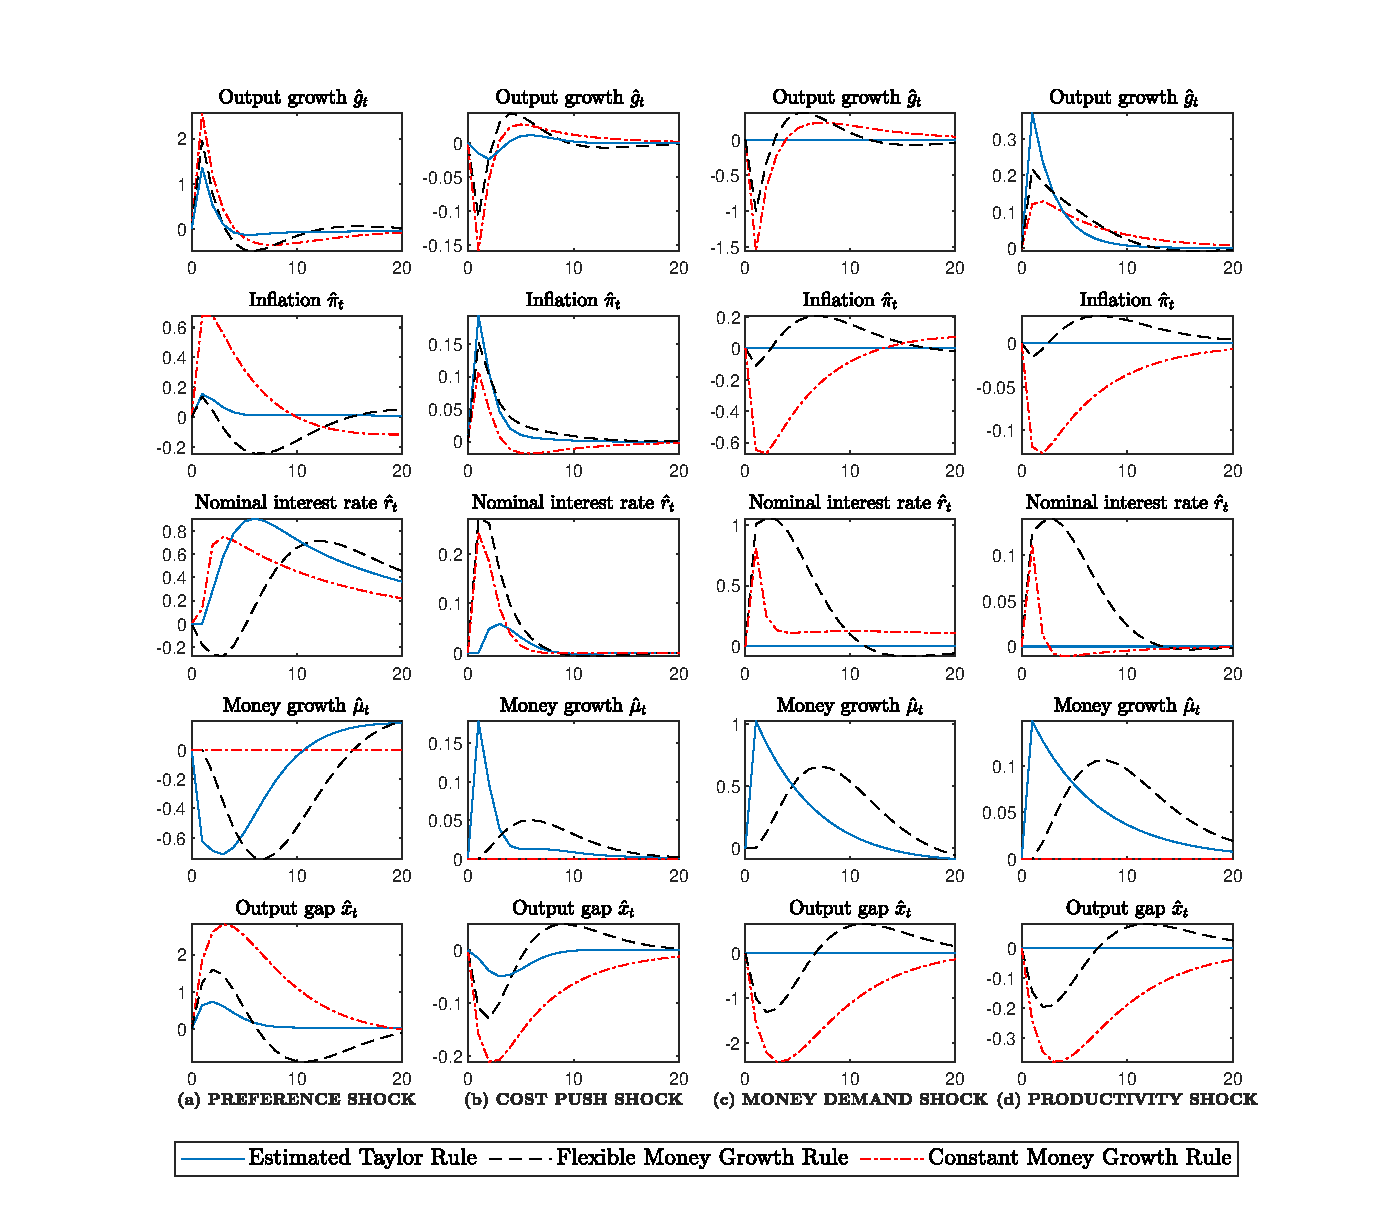
\includegraphics[width=1.2\textwidth]{code/final_irf_grid.eps}
  \caption{Impulse responses to the indicated shock under the benchmark sample. Each column shows the percentage-point response of the indicated variable to a one-standard-deviation $\sigma_i$,for $i=a_t, z_t, u_t, e_t$, under the estimated Taylor rule (\ref{s1}), the flexible money growth rule (\ref{s2}),and the constant money growth rule (\ref{s3}).}
  \label{irf1}
\end{figure}

\hypertarget{comparisson-to-constant-money-growth-rule}{%
\subsection{\texorpdfstring{Comparisson to constant money growth rule
(\ref{s3})}{Comparisson to constant money growth rule ()}}\label{comparisson-to-constant-money-growth-rule}}

The constant money growth rule (\ref{s3}) represents the case where
\(\rho_{mm} = \rho_{m \pi}= \rho_{mx}=0\) is applied to the flexible
money growth rule (\ref{s3}). Additionally, as motivated in section
\ref{data}, the (gross) constant money growth rate \(\hat{\mu}_t\) is
set equal to 1.0136 as in Ireland
(\protect\hyperlink{ref-ireland2011}{2011}). The estimated prior and
posterior distributions under the constant money growth rule by Ireland
(\protect\hyperlink{ref-ireland2000}{2000}), Collard \& Dellas
(\protect\hyperlink{ref-collard2005}{2005}), Gali
(\protect\hyperlink{ref-gali2015}{2015}), and Belongia \& Ireland
(\protect\hyperlink{ref-belongia2020}{2020}) indicate that macroeconomic
volatility would have been severely escalated if the Fed had followed a
constant money growth rule as specified here. Specifically, Belongia \&
Ireland (\protect\hyperlink{ref-belongia2020}{2020}) finds that median
estimates of the standard deviations of output growth and inflation are
more than \(50\) per cent larger under this constant money growth rule
than under the conventional Taylor rule. The impulse response functions
under this constant money growth rule, given in Figure \ref{irf1},
supports these authors' findings, and the analysis is discussed below.

In general, the efficacy of the constant money growth rule, simulated in
Figure \ref{irf1}, performs rather poorly, especially relative to both
the estimated Taylor and flexible money growth rules. The constant money
growth rule fails to exhibit the monetary tightening induced by both the
Taylor and flexible money growth rules. Therefore, output growth,
inflation, and the output gap under constant money growth illustrate
substantially more volatility in response to a preference shock column
\((a)\) of Figure \ref{irf1}.

Similarly, column \((d)\) of Figure \ref{irf1} shows that in response to
an accommodative productivity shock, the constant money growth rule is
absent of the gradual increase in money growth that facilitates an
efficient recovery in the economy evident in both the Taylor rule and
the flexible money growth rule. As a result, even though the output gap
and inflation are more volatile, output growth notably exhibits more
stability in the case of a constant money growth rule in response to a
productivity shock.

In stark contrast to the Taylor and flexible money growth rule, column
\((c)\) of Figure \ref{irf1} shows that the constant money growth rule
permits money demand shocks to exacerbate macroeconomic volatility.

Lastly, some positives can be drawn from column \((b)\) of Figure
\ref{irf1}, illustrating that the constant money growth rule performs
moderately better than the Taylor and flexible money growth rules in
stabilising inflation in response to a cost-push shock. However, this
inflation stability comes at the cost of permitting substantially more
significant output growth and output gap variability.

The literature consensus indicates that QE lowers longer-term interest
rates through a central bank balance sheet re-balancing channel on the
term premium, which in turn generates expansionary effects on output and
inflation (\protect\hyperlink{ref-borio2018}{Borio \& Zabai, 2018}; and
\protect\hyperlink{ref-carlson2020}{Carlson, D'Amico, Fuentes-Albero,
Schlusche \& Wood, 2020}). Therefore, assuming some combination of a
flexible or constant money growth rule and a rule for central bank open
market operations is undoubtedly attractive for future studies; however,
it is outside the scope of this project \footnote{See Gertler \& Karadi
  (\protect\hyperlink{ref-gertler2011}{2011}), Gertler \& Karadi
  (\protect\hyperlink{ref-gertler2018}{2018}), and Bernanke
  (\protect\hyperlink{ref-bernanke2020}{2020}) for possible QE rules
  that can be combined with money growth rules for monetary policy.}.

\hypertarget{analysis-of-results--estimated-smoothed-variables}{%
\section{Analysis of Results- Estimated Smoothed
Variables}\label{analysis-of-results--estimated-smoothed-variables}}

\begin{figure}
\centering
\hspace*{-1.5cm} 
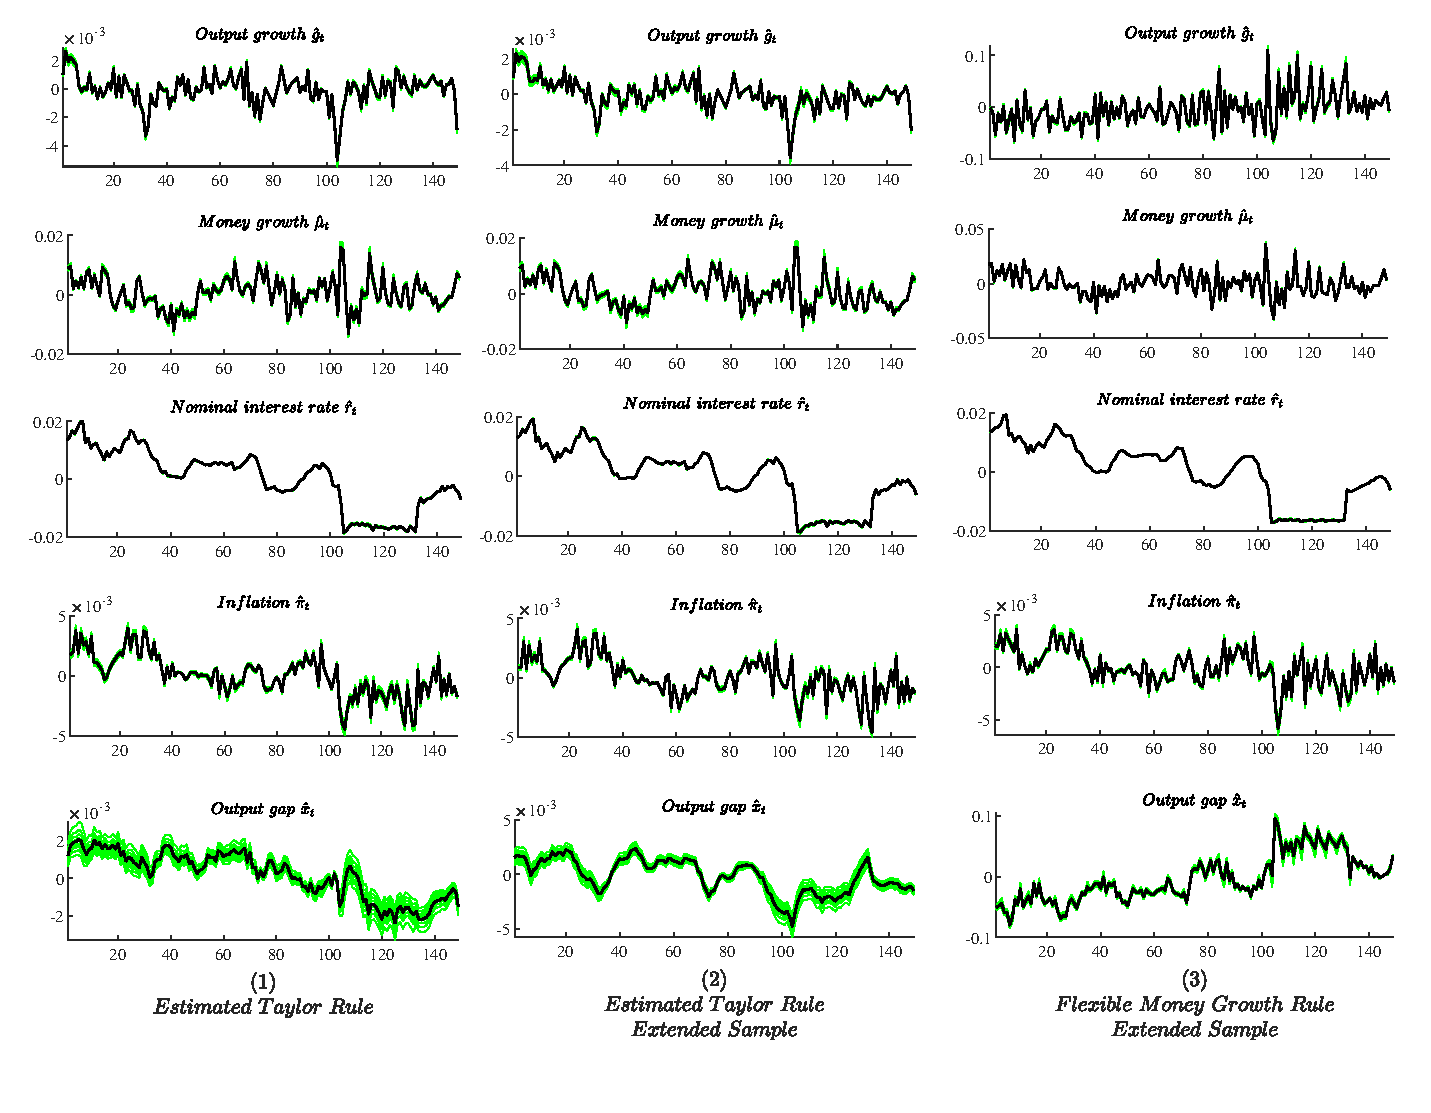
\includegraphics[width=1.2\textwidth]{code/1step_forecast.eps}
\caption{Smoothed variables –  The black line depicts the estimate of the smoothed variable (“best guess for the observed variable given all observations”), derived from the Kalman smoother at the posterior mean (Bayesian estimation). The green lines represent the deciles of the one step ahead forecast distribution.}
\label{smoothed}
\end{figure}

The Bayesian estimates of the smoothed variables (``best guess for the
observed variable given all observations''), derived from the Kalman
smoother at the posterior mean are shown in Figure \ref{smoothed} for
the benchmark sample Taylor rule, and the extended sample Taylor rule
and flexible money growth rule in columns \((1)\), \((2)\), and \((3)\),
respectively. Once the sample has been extended, the Taylor rule
performs similar than under the benchmark sample, with the exception of
exhibiting significantly less volatility in the output gap.

However, the main findings of Belongia \& Ireland
(\protect\hyperlink{ref-belongia2020}{2020}) are still apparent when the
sample is extended; The flexible money growth rule could have caused the
US economy to regain its strength quicker following the the 2008-9
recession, with a significantly shorter period of extraordinarily low
interest rates.

\hypertarget{conclusion}{%
\section{Conclusion}\label{conclusion}}

This project replicates model by Belongia \& Ireland
(\protect\hyperlink{ref-belongia2020}{2020}) using Bayesian estimation
techniques and performs simulation analysis with alternative monetary
policy rules, namely an estimated interest rate rule, a (flexible) money
supply rule, and a constant money supply rule. In addition, the sample
is extended, to verify the robustness of the authors' findings.

The estimated results are similar to that of Belongia \& Ireland
(\protect\hyperlink{ref-belongia2020}{2020}); impulse response
simulations, estimated using sample data from 1983:1 up to 2019:1 on the
US economy, show that a (flexible) money growth rule, whereby deviations
in the output gap are counteracted with modest and gradual changes to
the money growth rate, has efficacy levels comparable to the estimated
interest rate rule in stabilising output and inflation. Moreover, under
a constant money growth rule, output and inflation illustrate
substantially more volatility, consistent with the findings by Ireland
(\protect\hyperlink{ref-ireland2000}{2000}), Collard \& Dellas
(\protect\hyperlink{ref-collard2005}{2005}), and Gali
(\protect\hyperlink{ref-gali2015}{2015}).

Crucially, the findings of this project support Belongia \& Ireland
(\protect\hyperlink{ref-belongia2020}{2020})'s counterfactual
simulations, disclosing that the US economy would have recovered faster
from the crisis-induced recession under the same money growth rule and a
significantly shorter period of ground-level interest rates.
Additionally, the simulations presented here show that a money growth
rule has satisfactory performance in both the good and the bad times.
These findings iterate that the Fed, and other monetary authorities,
should consider money growth targeting as a strategy during periods
whereby the ZLB diminishes the historical and conventional method of
interest rate targeting.

\hypertarget{references}{%
\section*{References}\label{references}}
\addcontentsline{toc}{section}{References}

\hypertarget{refs}{}
\begin{CSLReferences}{1}{0}
\leavevmode\vadjust pre{\hypertarget{ref-beck2008}{}}%
Beck, G.W. \& Wieland, V. 2008. Central bank misperceptions and the role
of money in interest-rate rules. \emph{Journal of Monetary Economics}.
55:S1--S17.

\leavevmode\vadjust pre{\hypertarget{ref-bedard2008optimal}{}}%
Bedard, M. 2008. Optimal acceptance rates for metropolis algorithms:
Moving beyond 0.234. \emph{Stochastic Processes and their Applications}.
118(12):2198--2222.

\leavevmode\vadjust pre{\hypertarget{ref-belongia2018}{}}%
Belongia, M.T. \& Ireland, P.N. 2018. Targeting constant money growth at
the zero lower bound. \emph{53rd issue (March 2018) of the International
Journal of Central Banking}.

\leavevmode\vadjust pre{\hypertarget{ref-belongia2020}{}}%
Belongia, M.T. \& Ireland, P.N. 2020. A reconsideration of money growth
rules. \emph{Journal of Economic Dynamics and Control}. 104312.

\leavevmode\vadjust pre{\hypertarget{ref-bernanke2020}{}}%
Bernanke, B.S. 2020. The new tools of monetary policy. \emph{American
Economic Review}. 110(4):943--83.

\leavevmode\vadjust pre{\hypertarget{ref-borio2018}{}}%
Borio, C. \& Zabai, A. 2018. Unconventional monetary policies: A
re-appraisal. In Edward Elgar Publishing \emph{Research handbook on
central banking}.

\leavevmode\vadjust pre{\hypertarget{ref-brooks1998}{}}%
Brooks, S.P. \& Gelman, A. 1998. General methods for monitoring
convergence of iterative simulations. \emph{Journal of computational and
graphical statistics}. 7(4):434--455.

\leavevmode\vadjust pre{\hypertarget{ref-carlson2020}{}}%
Carlson, M.A., D'Amico, S., Fuentes-Albero, C., Schlusche, B. \& Wood,
P.R. 2020. Issues in the use of the balance sheet tool.

\leavevmode\vadjust pre{\hypertarget{ref-castelnuovo2012}{}}%
Castelnuovo, E. 2012. Estimating the evolution of money's role in the US
monetary business cycle. \emph{Journal of Money, Credit and Banking}.
44(1):23--52.

\leavevmode\vadjust pre{\hypertarget{ref-collard2005}{}}%
Collard, F. \& Dellas, H. 2005. Poole in the new keynesian model.
\emph{European Economic Review}. 49(4):887--907.

\leavevmode\vadjust pre{\hypertarget{ref-friedman1968}{}}%
Friedman, M. 1968. The role of monetary policy. \emph{Essential Readings
in Economics}. 58(1):215--231.

\leavevmode\vadjust pre{\hypertarget{ref-gali2015}{}}%
Gali, J. 2015. \emph{Monetary policy, inflation, and the business cycle:
An introduction to the new keynesian framework and its applications}.
Princeton University Press.

\leavevmode\vadjust pre{\hypertarget{ref-gertler2011}{}}%
Gertler, M. \& Karadi, P. 2011. A model of unconventional monetary
policy. \emph{Journal of monetary Economics}. 58(1):17--34.

\leavevmode\vadjust pre{\hypertarget{ref-gertler2018}{}}%
Gertler, M. \& Karadi, P. 2018. Qe 1 vs. 2 vs. 3...: A framework for
analyzing large-scale asset purchases as a monetary policy tool.
\emph{29th issue (January 2013) of the International Journal of Central
Banking}.

\leavevmode\vadjust pre{\hypertarget{ref-ireland2000}{}}%
Ireland, P.N. 2000. Expectations, credibility, and time-consistent
monetary policy. \emph{Macroeconomic Dynamics}. 4(4):448--466.

\leavevmode\vadjust pre{\hypertarget{ref-ireland2003}{}}%
Ireland, P.N. 2003. Technology shocks in the new keynesian model.
\emph{Review of Economics and Statistics}. 86(4):923--936.

\leavevmode\vadjust pre{\hypertarget{ref-ireland2011}{}}%
Ireland, P.N. 2011. A new keynesian perspective on the great recession.
\emph{Journal of Money, Credit and Banking}. 43(1):31--54.

\leavevmode\vadjust pre{\hypertarget{ref-piazzesi2019}{}}%
Piazzesi, M., Rogers, C. \& Schneider, M. 2019. Money and banking in a
new keynesian model. \emph{Standford WP}.

\leavevmode\vadjust pre{\hypertarget{ref-poole1970}{}}%
Poole, W. 1970. Optimal choice of monetary policy instruments in a
simple stochastic macro model. \emph{The Quarterly Journal of
Economics}. 84(2):197--216.

\leavevmode\vadjust pre{\hypertarget{ref-rupert2019}{}}%
Rupert, P. \& Šustek, R. 2019. On the mechanics of new-keynesian models.
\emph{Journal of Monetary Economics}. 102:53--69.

\leavevmode\vadjust pre{\hypertarget{ref-tarassow2019}{}}%
Tarassow, A. 2019. Forecasting US money growth using economic
uncertainty measures and regularisation techniques. \emph{International
Journal of Forecasting}. 35(2):443--457.

\leavevmode\vadjust pre{\hypertarget{ref-taylor1993}{}}%
Taylor, J.B. 1993. Discretion versus policy rules in practice. In Vol.
39. Elsevier \emph{Carnegie-rochester conference series on public
policy}. 195--214.

\leavevmode\vadjust pre{\hypertarget{ref-walsh2010}{}}%
Walsh, C.E. 2010. Central bank independence. In Springer \emph{Monetary
economics}. 21--26.

\leavevmode\vadjust pre{\hypertarget{ref-woodford2012}{}}%
Woodford, M. 2012. Methods of policy accommodation at the interest-rate
lower bound.

\end{CSLReferences}

\newpage
\appendix
\renewcommand{\thesection}{Appendix A}

\hypertarget{bayesian-esimation-results--taylor-rule-benchmark-sample}{%
\section{\texorpdfstring{Bayesian Esimation Results- Taylor Rule
(\ref{s1}), Benchmark Sample
\label{aa}}{Bayesian Esimation Results- Taylor Rule (), Benchmark Sample }}\label{bayesian-esimation-results--taylor-rule-benchmark-sample}}

\begin{figure}[H]
\includegraphics[width=0.8\linewidth,height=0.43\textheight]{code/png_images/priors_posteriors} \caption{Estimated posterior distributions (black solid line) for the benchmark sample under the Taylor rule. The grey line shows the prior density and the black line the density of the posterior distribution. The blue horizontal line indicates the posterior mode. \label{posterior1}}\label{fig:posteriors and priors}
\end{figure}

\begin{figure}
     \centering
     \begin{subfigure}[H]{0.49\textwidth}
         \centering
         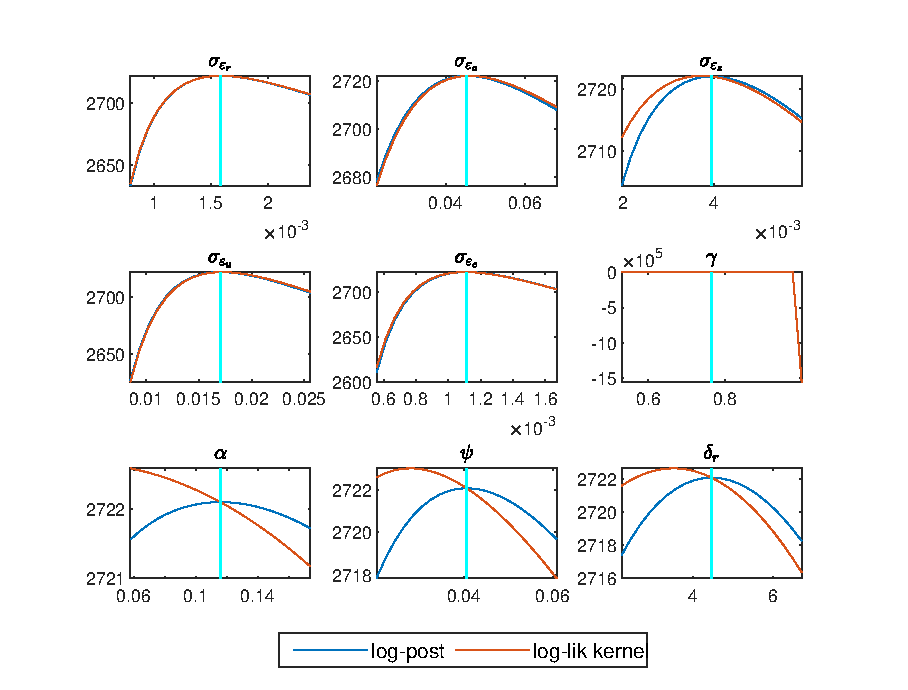
\includegraphics[width=\textwidth]{code/mode_check1}
     \end{subfigure}
     \begin{subfigure}[H]{0.49\textwidth}
         \centering
         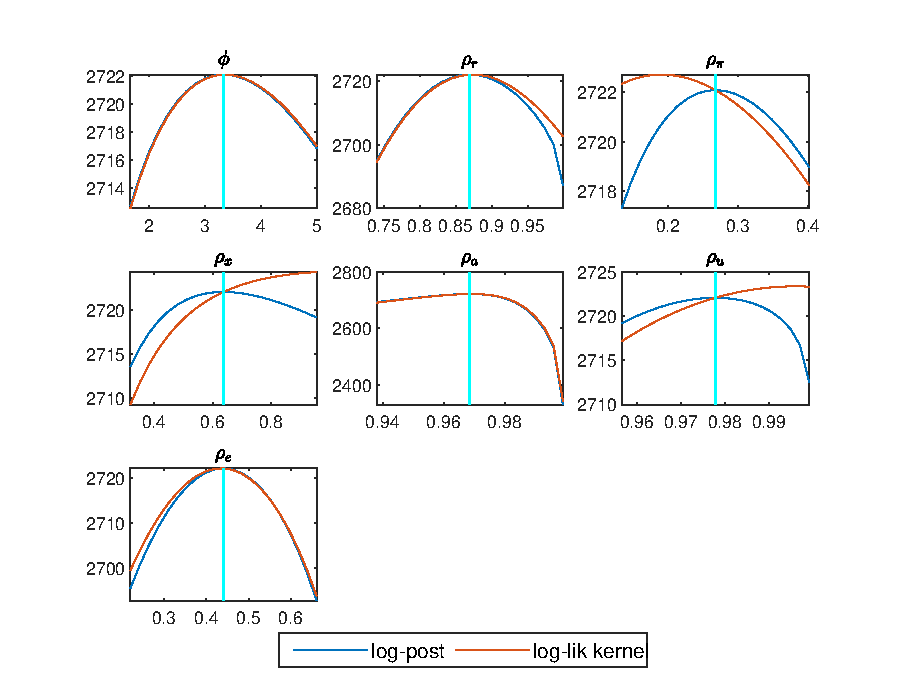
\includegraphics[width=\textwidth]{code/mode_check2}
     \end{subfigure}
        \caption{Estimated structural parameters mode check plots for benchmark sample under Taylor rule. The difference in the shapes of the likelihood kernel (red line) and the posterior likelihood
(blue line) indicates the role of the prior in influencing the curvature of the likelihood function.}
        \label{mc1}
\end{figure}

\begin{figure}
\centering
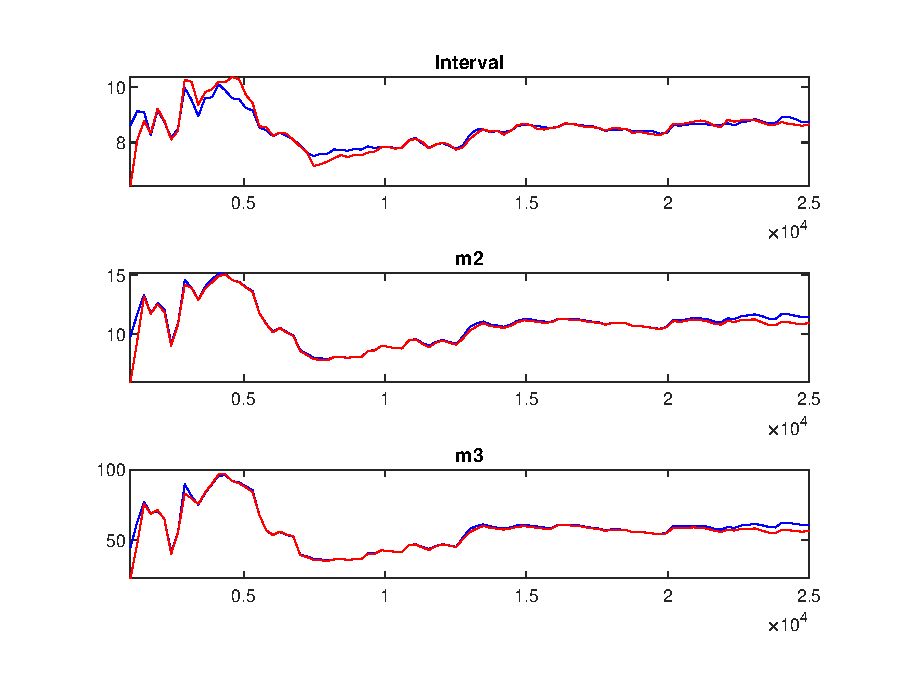
\includegraphics[width = 0.5\textwidth]{code/mcmc_m}
\caption{MCMC multivariate diagnostics of structural parameters for benchmark sample under the estimated Taylor rule [@brooks1998]. The first plot shows the convergence diagnostics for the 80 per cent interval. The second and third plots shows the estimates of the second and third central moments (m2 and m3), respectively. The red line shows the 80 per cent quantile range based on the 25 0000 pooled draws from all sequences and the blue line shows the mean interval range based on the draws of the individual sequences.}
\label{mcmcm1}
\end{figure}

\begin{figure}
     \centering
     \begin{subfigure}[H]{0.49\textwidth}
         \centering
         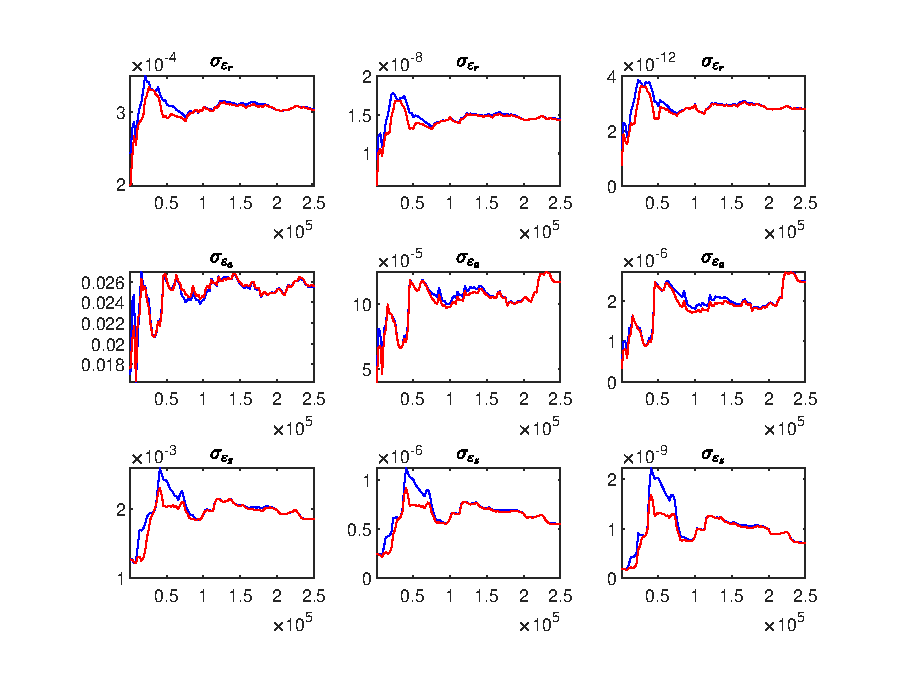
\includegraphics[width=\textwidth]{code/mcmc_u1}
     \end{subfigure}
     \begin{subfigure}[H]{0.49\textwidth}
         \centering
         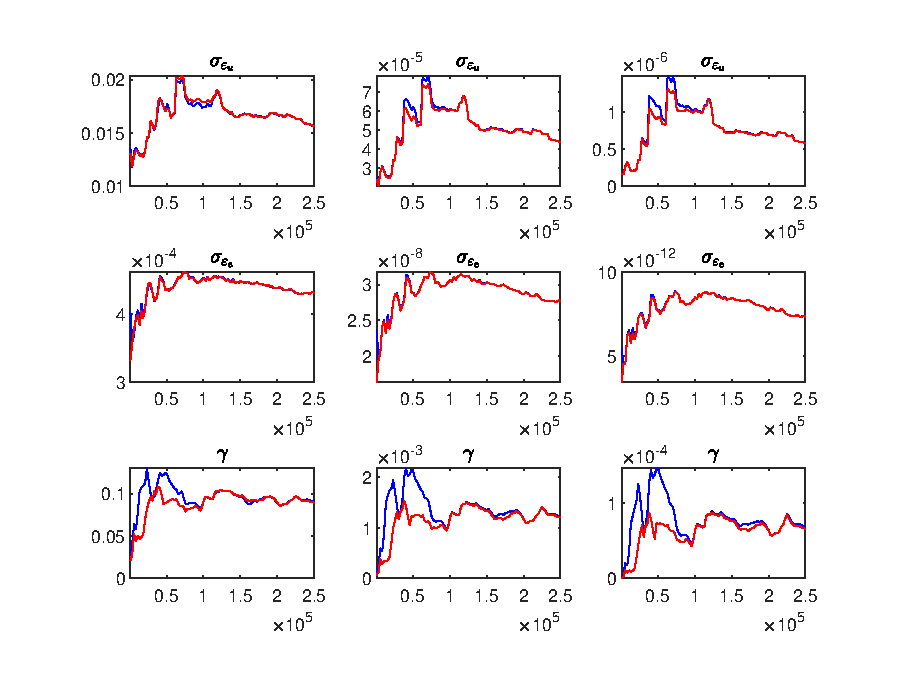
\includegraphics[width=\textwidth]{code/mcmc_u2}
     \end{subfigure}
    \begin{subfigure}[H]{0.49\textwidth}
         \centering
         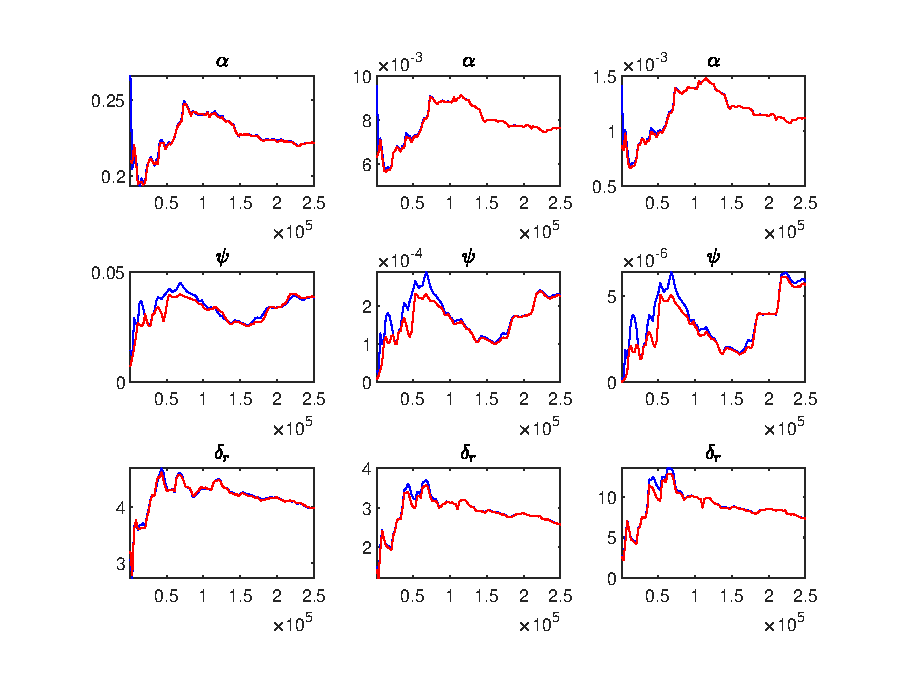
\includegraphics[width=\textwidth]{code/mcmc_u3}
     \end{subfigure}
    \begin{subfigure}[H]{0.49\textwidth}
         \centering
         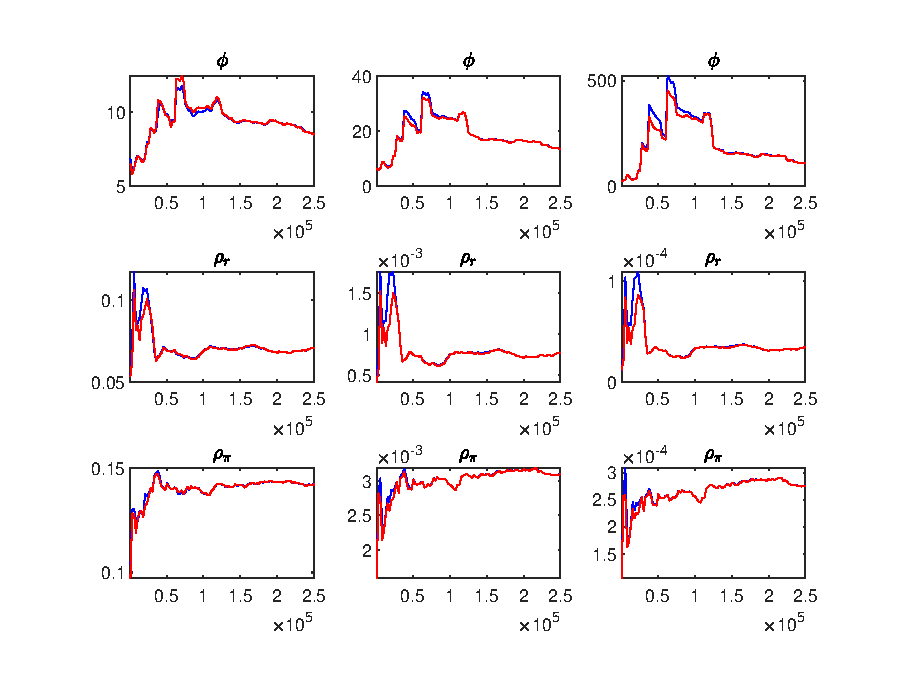
\includegraphics[width=\textwidth]{code/mcmc_u4}
     \end{subfigure}
    \begin{subfigure}[H]{0.49\textwidth}
         \centering
         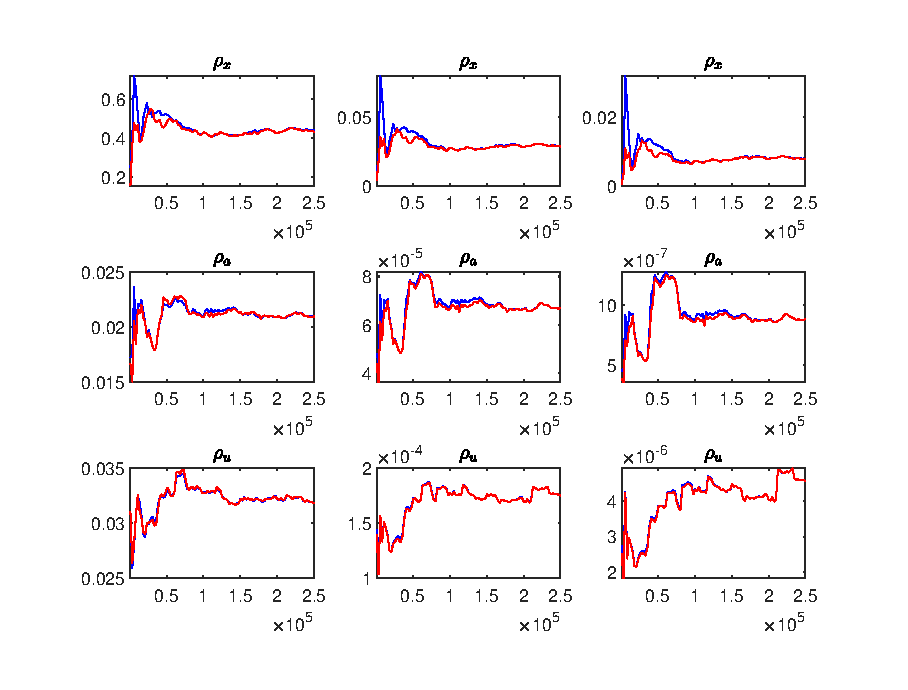
\includegraphics[width=\textwidth]{code/mcmc_u5}
     \end{subfigure}
      \begin{subfigure}[H]{0.49\textwidth}
         \centering
         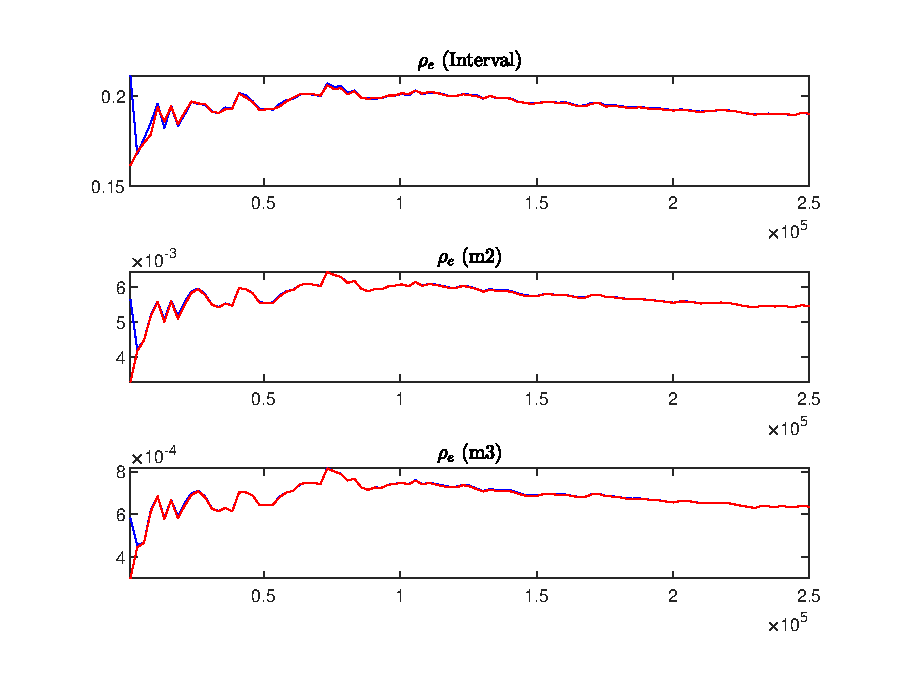
\includegraphics[width=\textwidth]{code/mcmc_u6}
     \end{subfigure}
        \caption{MCMC univariate diagnostics of structural parameters for extended sample under estimated the Taylor rule (\ref{s1}) [@brooks1998]. For each parameter, the first column shows the convergence diagnostics for the 80 per cent interval. The second and third columns shows the estimates of the second and third central moments (m2 and m3), respectively. The red line shows the 80 per cent quantile range based on the 25 000 pooled draws from all sequences and the blue line shows the mean interval range based on the draws of the individual sequences.}
        \label{mcmcu1}
\end{figure}

\newpage
\renewcommand{\thesection}{Appendix B}

\hypertarget{bayesian-esimation-results--taylor-rule-extended-sample}{%
\section{\texorpdfstring{Bayesian Esimation Results- Taylor Rule
(\ref{s1}) , Extended Sample
\label{bb}}{Bayesian Esimation Results- Taylor Rule () , Extended Sample }}\label{bayesian-esimation-results--taylor-rule-extended-sample}}

\begin{figure}
     \centering
     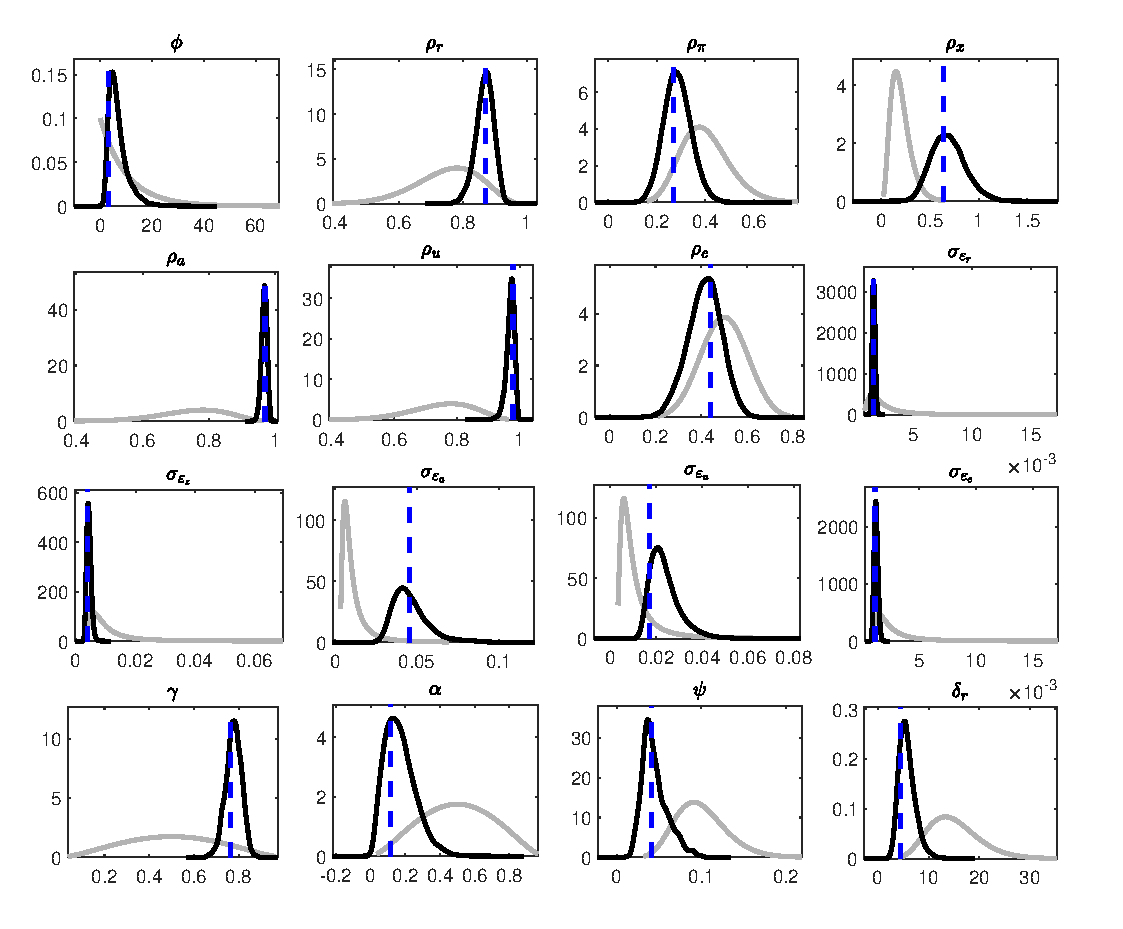
\includegraphics[height=0.4\textheight]{code/posterior_extended.eps}
    \caption{Estimated posterior distributions (black solid line) for the extended sample under the Taylor rule. The grey line shows the prior density and the black line the density of the posterior distribution. The blue horizontal line indicates the posterior mode.}
        \label{posterior_extended1}
\end{figure}

\begin{figure}
     \centering
     \begin{subfigure}[H]{0.49\textwidth}
         \centering
         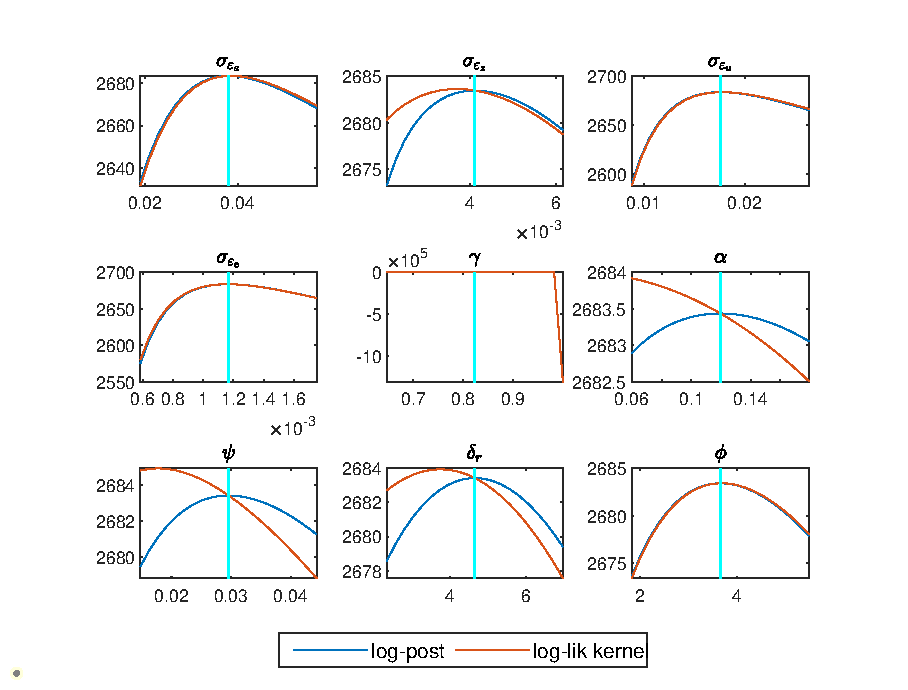
\includegraphics[width=\textwidth]{code/mode_check1_extended}
     \end{subfigure}
     \begin{subfigure}[H]{0.49\textwidth}
         \centering
         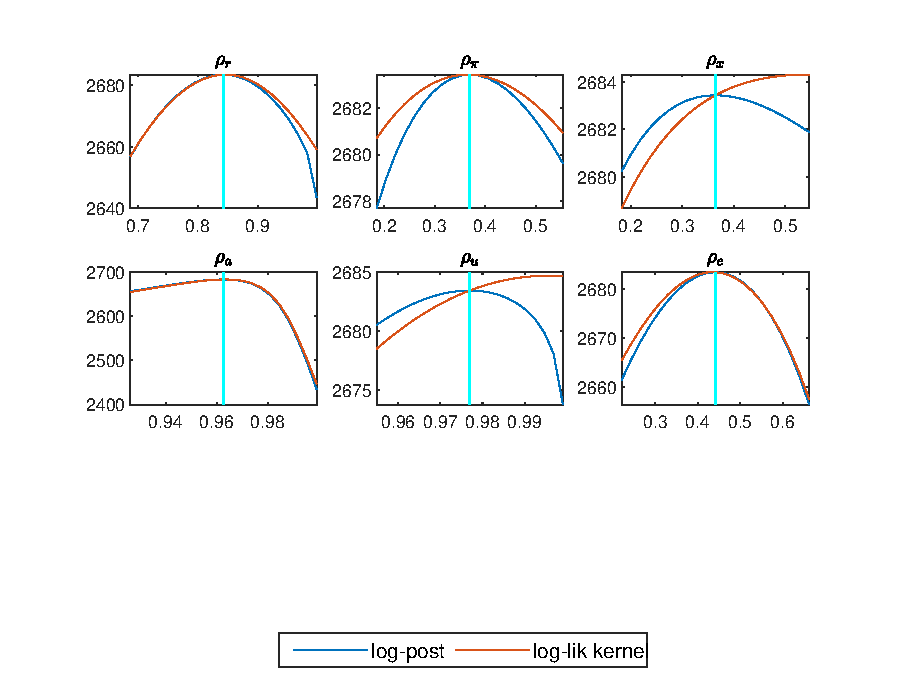
\includegraphics[width=\textwidth]{code/mode_check2_extended}
     \end{subfigure}
        \caption{Estimated structural parameters mode check plots for extended sample under the Taylor rule (\ref{s1}). The difference in the shapes of the likelihood kernel (red line) and the posterior likelihood (blue line) indicates the role of the prior in influencing the curvature of the likelihood function.}
        \label{mc2}
\end{figure}

\begin{figure}
\centering
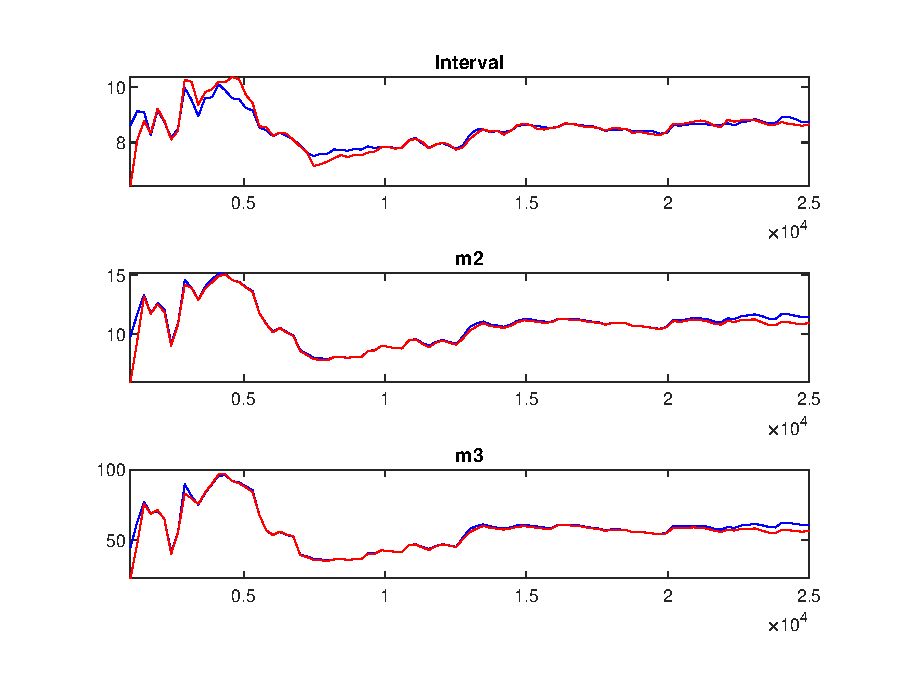
\includegraphics[width = 0.5\textwidth]{code/mcmc_m}
\caption{MCMC multivariate diagnostics of structural parameters for extended sample under the Taylor rule (\ref{s1}) [@brooks1998]. The first plot shows the convergence diagnostics for the 80 per cent interval. The second and third plots shows the estimates of the second and third central moments (m2 and m3), respectively. The red line shows the 80 per cent quantile range based on the 25 000 pooled draws from all sequences and the blue line shows the mean interval range based on the draws of the individual sequences.}
\label{mcmcm2}
\end{figure}

\begin{figure}
     \centering
     \begin{subfigure}[H]{0.49\textwidth}
         \centering
         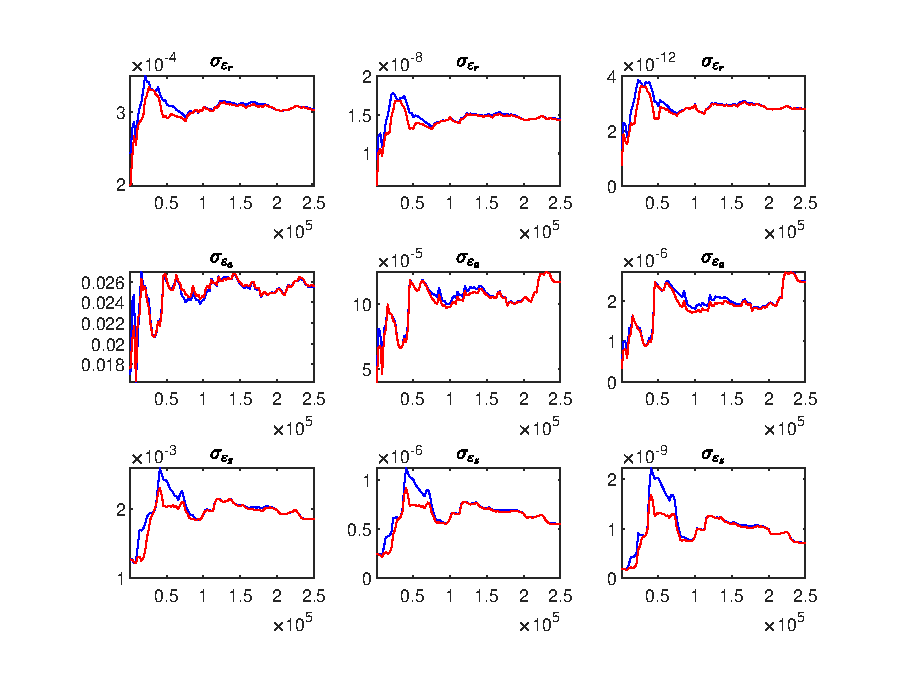
\includegraphics[width=\textwidth]{code/mcmc_u1}
     \end{subfigure}
     \begin{subfigure}[H]{0.49\textwidth}
         \centering
         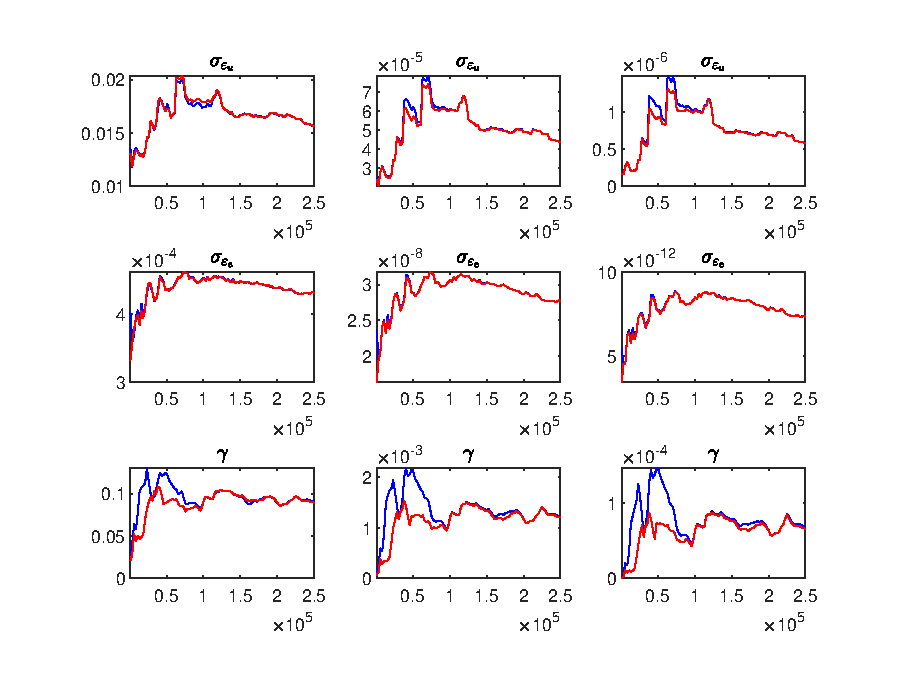
\includegraphics[width=\textwidth]{code/mcmc_u2}
     \end{subfigure}
    \begin{subfigure}[H]{0.49\textwidth}
         \centering
         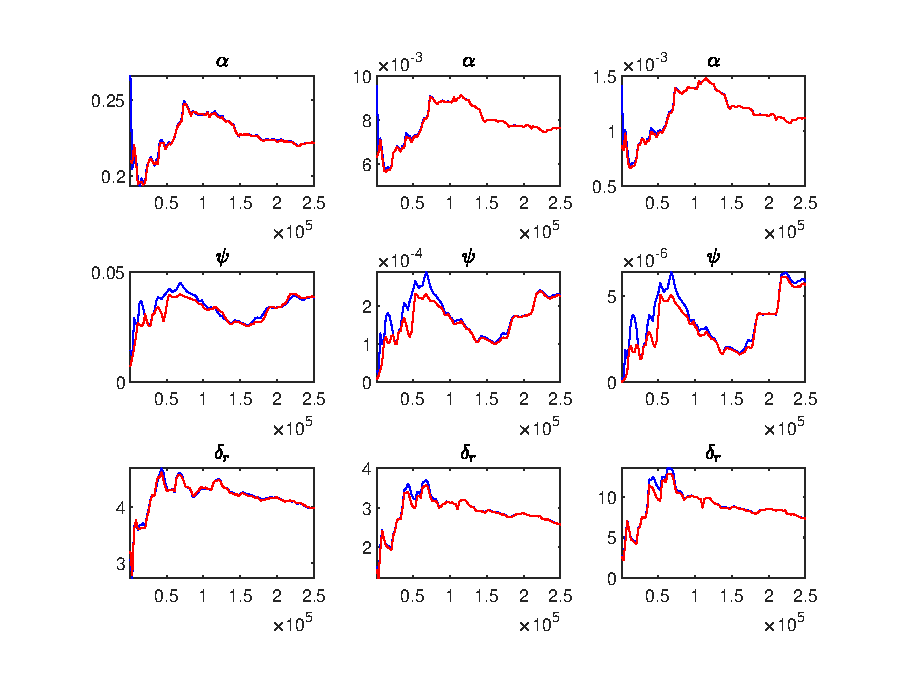
\includegraphics[width=\textwidth]{code/mcmc_u3}
     \end{subfigure}
    \begin{subfigure}[H]{0.49\textwidth}
         \centering
         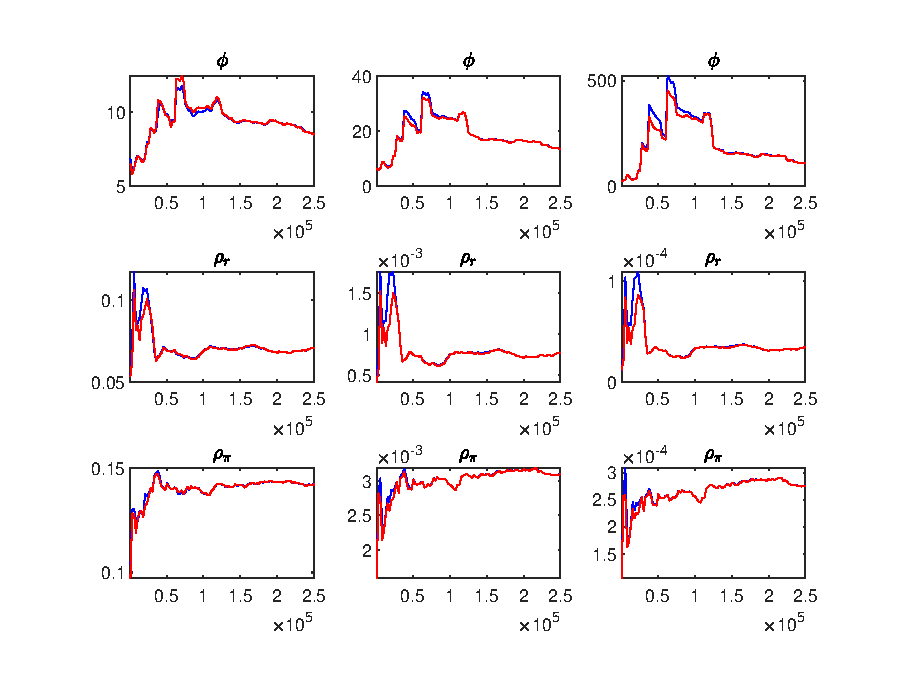
\includegraphics[width=\textwidth]{code/mcmc_u4}
     \end{subfigure}
    \begin{subfigure}[H]{0.49\textwidth}
         \centering
         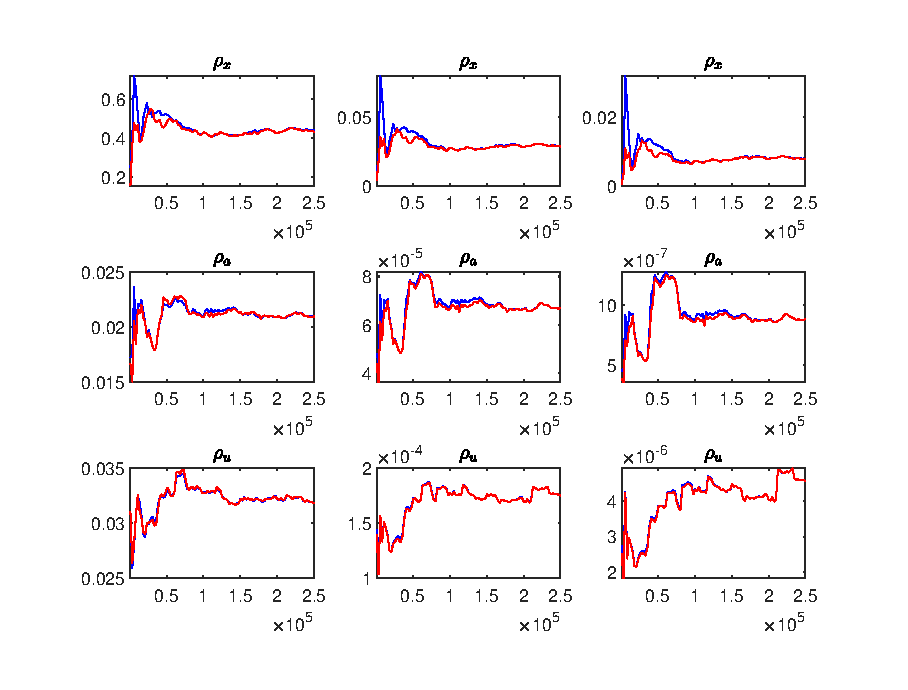
\includegraphics[width=\textwidth]{code/mcmc_u5}
     \end{subfigure}
      \begin{subfigure}[H]{0.49\textwidth}
         \centering
         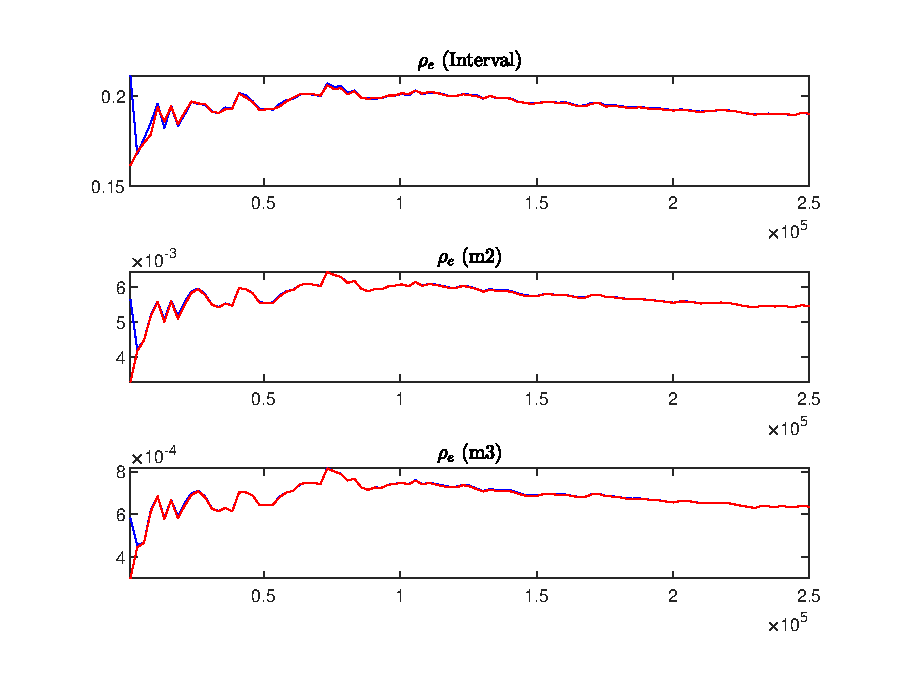
\includegraphics[width=\textwidth]{code/mcmc_u6}
     \end{subfigure}
        \caption{MCMC univariate diagnostics of structural parameters for extended sample under the estimated Taylor rule [@brooks1998]. For each parameter, the first column shows the convergence diagnostics for the 80 per cent interval. The second and third columns shows the estimates of the second and third central moments (m2 and m3), respectively. The red line shows the 80 per cent quantile range based on the pooled draws from all sequences and the blue line shows the mean interval range based on the 25 000 draws of the individual sequences.}
        \label{mcmcu2}
\end{figure}

\begin{figure}
  \centering
    \hspace*{-2cm}  
  \includegraphics[width=1.2\textwidth]{code/final_irf_grid_extended.eps}
  \caption{Impulse responses to the indicated shock under the extended sample. Each column shows the percentage-point response of the indicated variable to a one-standard-deviation $\sigma_i$,for $i=a_t, z_t, u_t, e_t$, under the estimated taylor rule (\ref{s1}) and the flexible money growth rule (\ref{s2}).}
  \label{irf2}
\end{figure}

\renewcommand{\thesection}{Appendix C}

\hypertarget{bayesian-esimation-results--flexible-money-growth-rule-extended-sample}{%
\section{\texorpdfstring{Bayesian Esimation Results- Flexible Money
Growth Rule (\ref{s2}), Extended Sample
\label{cc}}{Bayesian Esimation Results- Flexible Money Growth Rule (), Extended Sample }}\label{bayesian-esimation-results--flexible-money-growth-rule-extended-sample}}

\begin{figure}
     \centering
     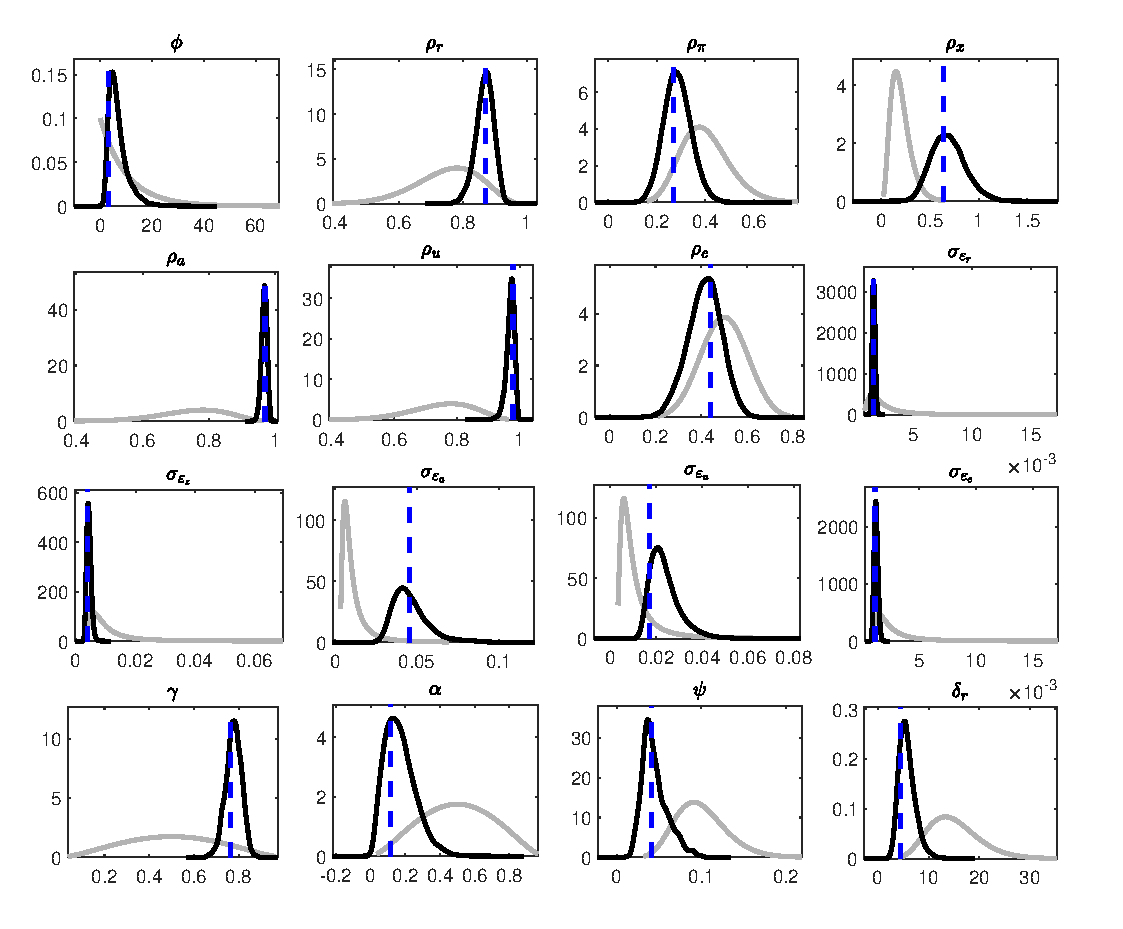
\includegraphics[height=0.4\textheight]{code/posterior_extended.eps}
    \caption{Estimated posterior distributions (black solid line) for the extended sample under the flexible money growth rule (\ref{s2}). The grey line shows the prior density and the black line the density of the posterior distribution. The blue horizontal line indicates the posterior mode.}
        \label{posterior_extended2}
\end{figure}

\begin{figure}
     \centering
     \begin{subfigure}[H]{0.49\textwidth}
         \centering
         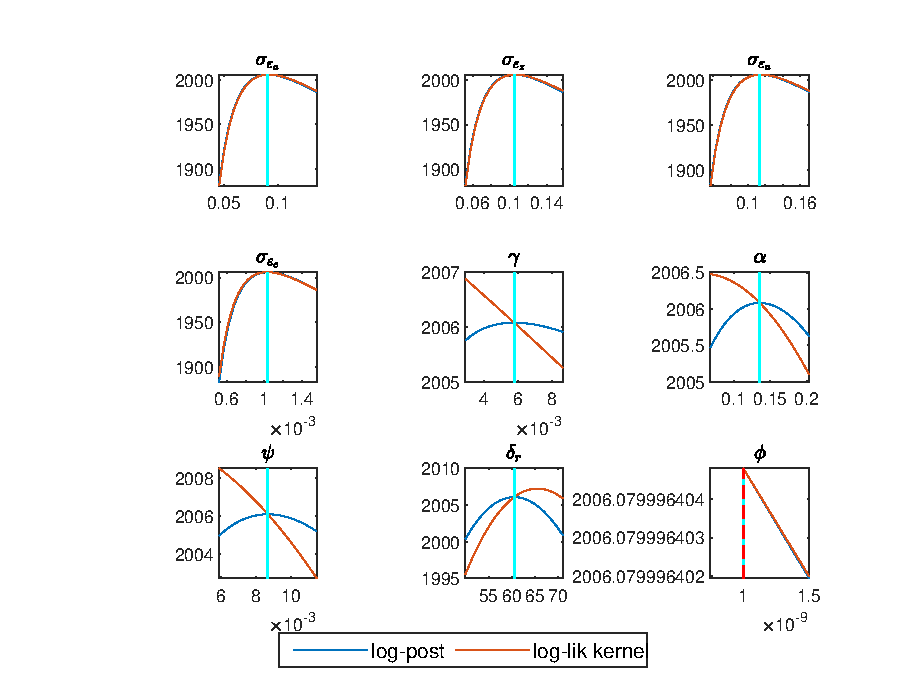
\includegraphics[width=\textwidth]{code/mode_check_1_money}
     \end{subfigure}
     \begin{subfigure}[H]{0.49\textwidth}
         \centering
         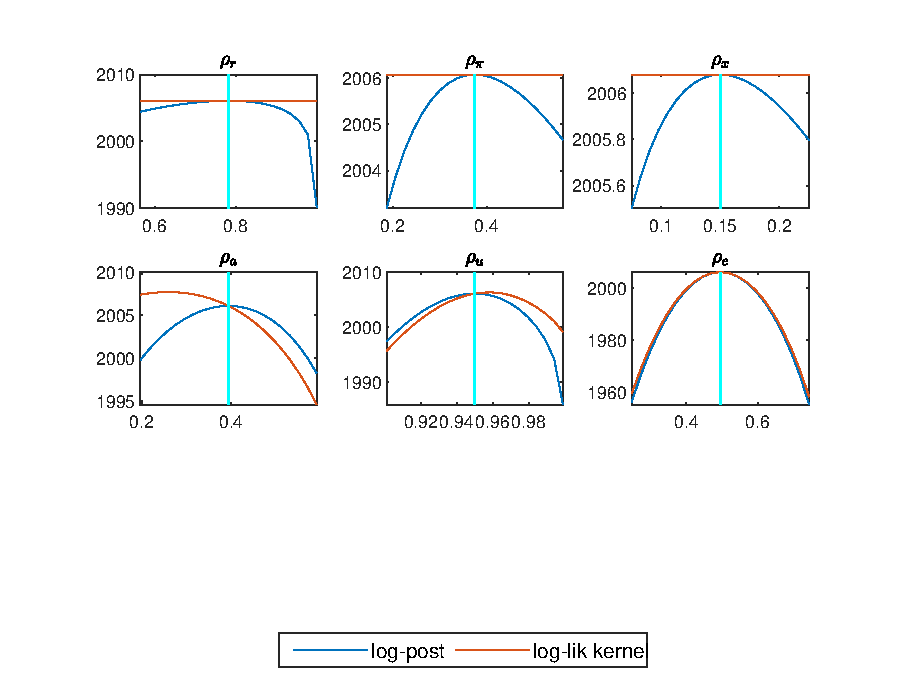
\includegraphics[width=\textwidth]{code/mode_check_2_money}
     \end{subfigure}
        \caption{Estimated structural parameters mode check plots for extended sample under flexible money growth rule (\ref{s2}). The difference in the shapes of the likelihood kernel (red line) and the posterior likelihood (blue line) indicates the role of the prior in influencing the curvature of the likelihood function.}
        \label{mc3}
\end{figure}

\begin{figure}
\centering
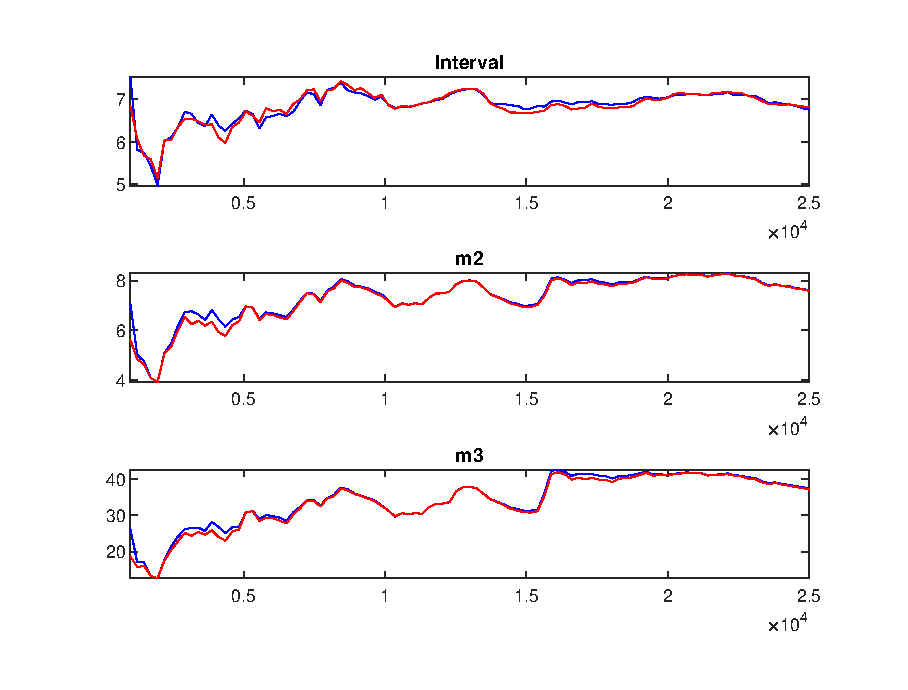
\includegraphics[width = 0.5\textwidth]{code/MCMC_m_money}
\caption{MCMC multivariate diagnostics of structural parameters for extended sample under the flexible money growth rule (\ref{s2}) [@brooks1998]. The first plot shows the convergence diagnostics for the 80 per cent interval. The second and third plots shows the estimates of the second and third central moments (m2 and m3), respectively. The red line shows the 80 per cent quantile range based on the 25 0000 pooled draws from all sequences and the blue line shows the mean interval range based on the draws of the individual sequences.}
\label{mcmcm3}
\end{figure}

\begin{figure}
     \centering
     \begin{subfigure}[H]{0.49\textwidth}
         \centering
         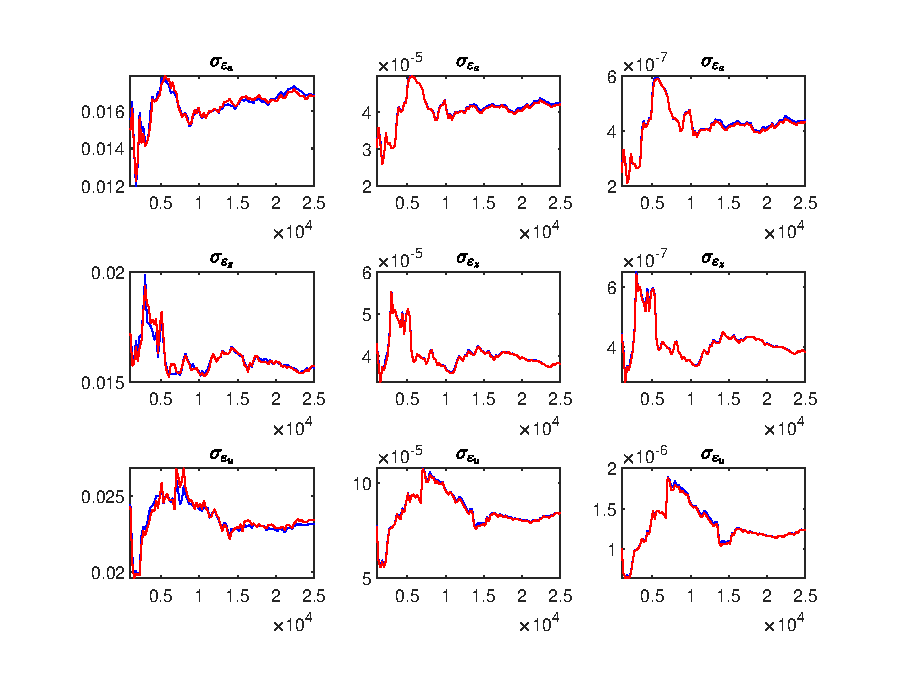
\includegraphics[width=\textwidth]{code/MCMC_1_money}
     \end{subfigure}
     \begin{subfigure}[H]{0.49\textwidth}
         \centering
         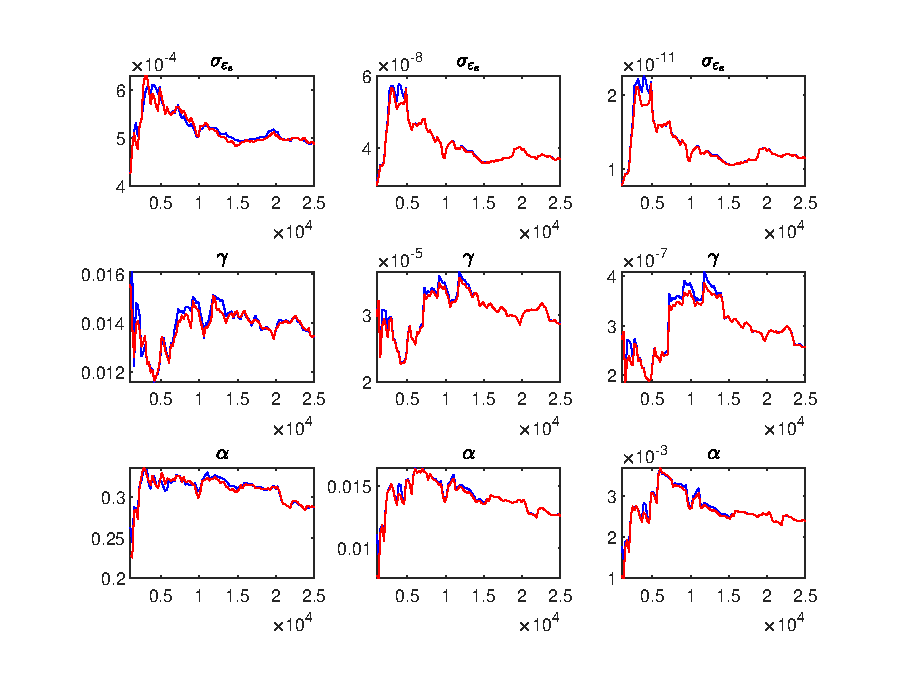
\includegraphics[width=\textwidth]{code/MCMC_2_money}
     \end{subfigure}
    \begin{subfigure}[H]{0.49\textwidth}
         \centering
         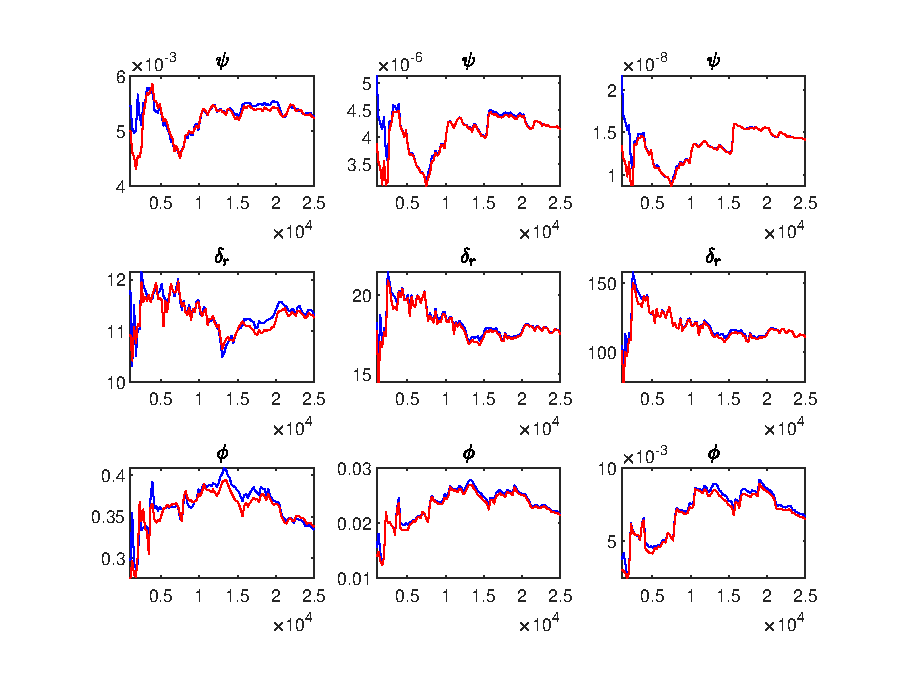
\includegraphics[width=\textwidth]{code/MCMC_3_money}
     \end{subfigure}
    \begin{subfigure}[H]{0.49\textwidth}
         \centering
         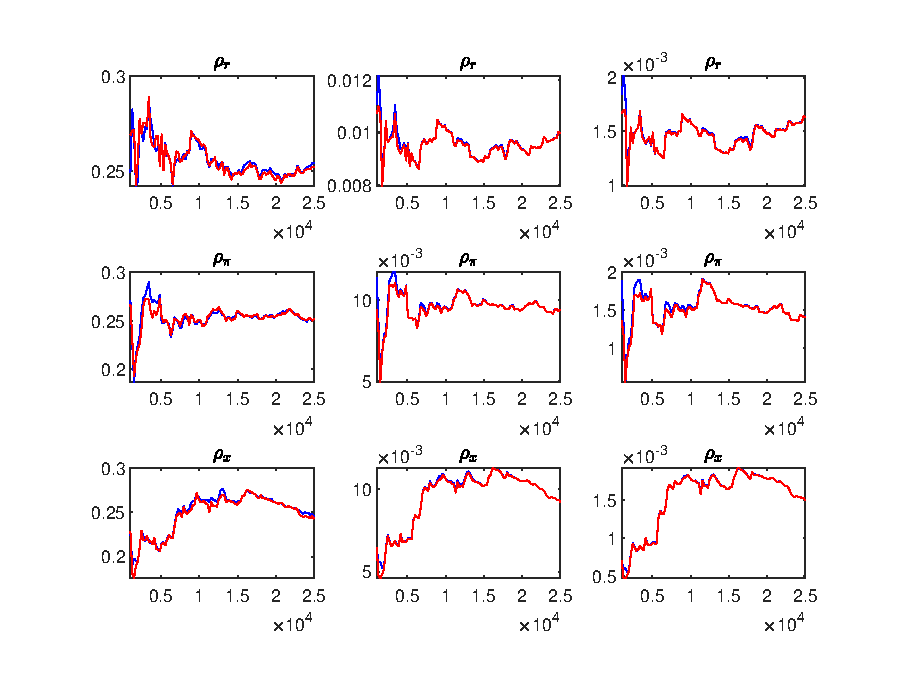
\includegraphics[width=\textwidth]{code/MCMC_4_money}
     \end{subfigure}
    \begin{subfigure}[H]{0.49\textwidth}
         \centering
         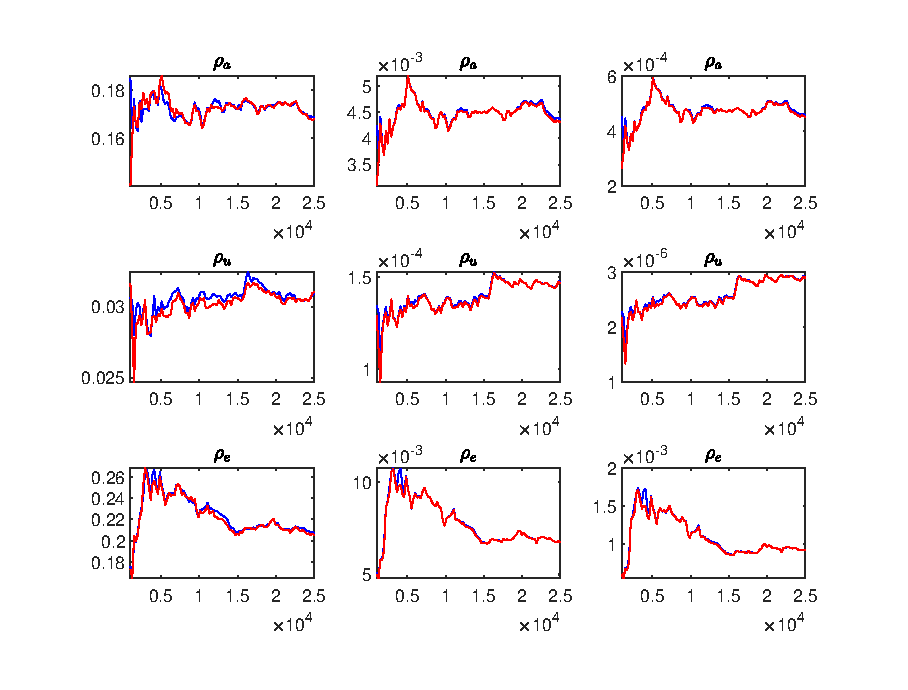
\includegraphics[width=\textwidth]{code/MCMC_5_money}
     \end{subfigure}
        \caption{MCMC univariate diagnostics of structural parameters for extended sample under the flexible money growth rule (\ref{s2}) [@brooks1998]. For each parameter, the first column shows the convergence diagnostics for the 80 per cent interval. The second and third columns shows the estimates of the second and third central moments (m2 and m3), respectively. The red line shows the 80 per cent quantile range based on the pooled draws from all sequences and the blue line shows the mean interval range based on 25 000 the draws of the individual sequences.}
        \label{mcmcu3}
\end{figure}

\bibliography{Tex/ref}





\end{document}
